\documentclass[11pt, a4paper, twoside, openright]{report}

\usepackage[]{graphicx}
\usepackage{tabularx}
\usepackage{subfigure}
\usepackage{afterpage}
\usepackage{amsmath,amssymb}            
\usepackage{rotating}  
\usepackage{fancyhdr}  
\usepackage{mathtools}
\usepackage[scriptsize]{caption} 
\usepackage{IEEEtrantools}
\usepackage{algorithm}
\usepackage{algorithmic}
\usepackage{multirow}
\hyphenation{ev-ery-where}

% ---- Custom defined envs and commands ----
\newtheorem{theorem}{Theorem}

\setlength{\paperwidth}{16cm}
\setlength{\paperheight}{24cm}
\setlength{\oddsidemargin} {1. cm}
\setlength{\evensidemargin} {1. cm}
\addtolength{\oddsidemargin} {-0.4 cm}
\addtolength{\evensidemargin} {-0.4 cm}
\addtolength{\textwidth}{2 cm}
\linespread{1.1}

\usepackage[english]{babel}
\usepackage[latin1]{inputenc}
\renewcommand{\captionfont}{\normalfont \sffamily \itshape \small}

\pagestyle{empty}

\begin{document}
% ---- Frontispiece ----
\thispagestyle{empty}
\vspace*{-1.5cm} \bfseries{
    \begin{center}
	\large
	POLITECNICO DI MILANO\\
	\normalsize
	Master's Degree in Computer Science and Engineering\\
	Dipartimento di Elettronica, Informazione e Bioingegneria\\
	    
	\vspace{0.6cm}
	
	\begin{figure}[htbp]
	    \begin{center}
	    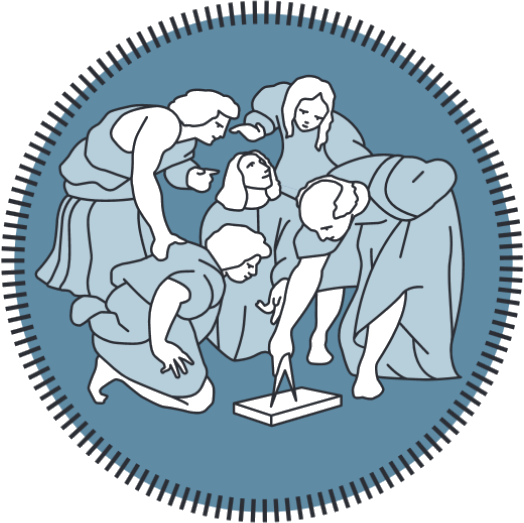
\includegraphics[width=3.5cm]{pictures/logopm}
	    \end{center}
	\end{figure}
	
	\vspace*{0.3cm} \LARGE

	\textbf{DEEP FEATURE EXTRACTION FOR SAMPLE-EFFICIENT REINFORCEMENT LEARNING}\\

	\vspace*{.75truecm} \large
    \end{center}

    \vspace*{3.0cm} \large

    \begin{flushleft}
	Supervisor: Prof.\ Marcello Restelli \\
	Co-supervisors: Dott.\ Carlo D'Eramo, Dott.\ Matteo Pirotta
    \end{flushleft}

    \vspace*{1.0cm}

    \begin{flushright}
	Master's Thesis by:\\ Daniele Grattarola (Student ID 853101)
    \end{flushright}

    \vspace*{0.5cm}

    \begin{center}
	Academic Year 2016-2017
    \end{center} \clearpage
}

\thispagestyle{empty} \normalfont \cleardoublepage

% ---- Dedication ----
\vspace{17cm}

\begin{flushright}
    \itshape{Il pi\`u \`e fatto.}
\end{flushright}

\thispagestyle{empty}  \cleardoublepage

\pagenumbering{Roman}

% ---- TOC ----
\tableofcontents
\listoffigures
\listoftables
\listofalgorithms

% ---- Summary ----
\newpage
\chapter*{Abstract}

\addcontentsline{toc}{chapter}{Abstract}

\vspace{0.5cm}

Deep reinforcement learning (DRL) has been under the spotlight of artificial 
intelligence research in recent years, enabling reinforcement learning agents 
to solve control problems that were previously considered intractable. 
The most effective DRL methods, however, require a great amount of training 
samples (in the order of tens of millions) in order to learn good policies
even on simple environments, making them a poor choice in real-world situations
where the collection of samples is expensive.

In this work, we propose a sample-efficient DRL algorithm that combines 
unsupervised deep learning to extract a representation of the environment, and 
batch reinforcement learning to learn a control policy using this new state 
space.
We also add an intermediate step of feature selection on the extracted 
representation in order to reduce the computational requirements of our agent to 
the minimum.
We test our algorithm on the Atari games environments, and compare the 
performance of our agent to that of the DQN algorithm by Mnih et al.\ \cite{mnih2015human}.
We show that even if the final performance of our agent amounts to a quarter of 
DQN's, we are able to achieve good sample efficiency and a better performance on
small datasets.
\newpage
\chapter*{Riassunto}

\addcontentsline{toc}{chapter}{Riassunto}



\thispagestyle{empty} \vspace*{.75truecm} \cleardoublepage

% ---- Acknowledgments ----
\chapter*{Acknowledgments}

\addcontentsline{toc}{chapter}{Aknowledgments}


All the work presented in this thesis was done under the supervision of 
Prof.\ Marcello Restelli, who has instilled in me the passion for this complex 
and fascinating subject and helped me navigate it for the best part of a year. 
I also thank Dott.\ Carlo D'Eramo and Dott.\ Matteo Pirotta for guiding 
me during my first steps into the academic world and inspiring me to pursue a 
career in research. 
It is impossible to summarize the unique experience I had at PoliMi in a few
paragraphs, but I would like to thank Ilyas Inajjar, Giacomo Locci, Angelo 
Gallarello, Davide Conficconi, Alessandro Comodi, Francesco Lattari, Edoardo
Longo, Stefano Longari, Yannick Giovanakis, Paolo Mosca and Andrea Lui for 
sharing their experiences with me and always showing me a different perspective
of the things we do. 
I thank Politecnico di Milano for providing the infrastructure during my education
and the writing of this thesis, but most importantly for fostering a culture 
of academic excellence, of collaboration, and of passion for the disciplines
of its students.
I also thank Prof.\ Cremonesi and Prof.\ Alippi for giving me a chance to prove 
myself.

Finally, this thesis is dedicated to my parents, for giving me all that I am and
all that I have; 
to Gaia, for being the reason to always look ahead;
to my grandmothers, for their unconditional love; 
to my grandfather, for always rooting silently.
\thispagestyle{empty} \vspace*{.75truecm} \normalfont \cleardoublepage

% ---- Style setup for main body ----
\pagestyle{plain}\renewcommand{\chaptermark}[1]{\markboth{\chaptername\ \thechapter.\ #1}{}} 
\renewcommand{\sectionmark}[1]{\markright{\thesection.\ #1}}         
\fancyhead[LE,RO]{\bfseries\thepage}    
                                        
\fancyhead[RE]{\bfseries\leftmark}    
\fancyhead[LO]{\bfseries\rightmark}     
\renewcommand{\headrulewidth}{0.3pt} 

\pagenumbering{arabic}

% ---- Main body ----
\chapter{Introduction}
\label{ch1_intro}
\thispagestyle{empty}

\vspace{0.5cm}
 
Human behavior is a complex mix of elements. We are subject to 
well defined biological and social forces, but at the same time our actions are 
deliberate, our thinking is abstract, and our objectives can be irrational; 
our brains are extremely complex interconnections, but of extremely simple 
building blocks; we are crafted by ages of random evolution, but at the same 
time of precise optimization. 
When we set out to describe the inner workings of human cognition, we must 
consider all of these colliding aspects and account for them in our work, 
without overcomplicating what is simple or approximating what is complex.

Artificial intelligence is a broad field, which looks at the variegate spectrum 
of human behavior to replicate our complexity in a formal or algorithmic way. 
Among the techniques of AI, one family of algorithms called \textit{machine
learning} is designed to give computers the ability to \textit{learn} to carry 
out a task without being explicitly programmed to do so. 
The focus on different types of tasks is what defines the many subfields of 
machine learning.
For instance, the use of machine learning algorithms to take decisions in a 
\textit{sequential decision-making problem} is called \textit{reinforcement 
learning}, whereas \textit{deep learning} is a family of techniques to learn an 
abstract representation of a vector space (e.g.\, learning how to describe an
image from the value of its pixels).

Teaching machines to behave like human beings is a complex and inspiring problem
on its own; however, an even more complex task is not to simply teach 
computers to mimic humans, but to do so with the same learning 
\textit{efficiency} of the biological brain, which is able to solve problems by
experiencing them very few times (sometimes even imagining a problem is enough 
to solve it, by comparing it with other similar known situations). 
The purpose of this thesis is to make a step in this direction by
combining powerful machine learning techniques with efficient ones, in order
to tackle complex control problems without needing many examples to learn
from.

\section{Goals and motivation}
The source of inspiration for this work comes from the recent progress in 
reinforcement learning associated to \textit{deep reinforcement learning} (DRL)
techniques. 
Among these, we cite \textit{Deep Q-Learning} by Mnih et al.\ \cite{mnih2015human},
the \textit{Asynchronous Advantage Actor-Critic} algorithm also by Mnih et 
al.\ \cite{mnih2016asynchronous}, and the \textit{Neural Episodic Control} 
algorithm by Pritzel et al.\ \cite{pritzel2017neural}.
All these algorithms (which were all the state of the art at the time of
their respective publication), are based on deep learning to extract 
the visual characteristics of an environment, and then using those 
characteristics to learn a policy with well-known reinforcement learning 
techniques. A major drawback of these approaches, however, is that they all 
require an enormous amount of experience to converge, which may prove unfeasible
in real-world problems where the collection of examples is expensive.
The main purpose of this work is to explore the limits of this apparent 
requirement, and to propose an algorithm that is able to perform well even under 
such scarcity conditions.

\section{Proposed solution}
We introduce a deep reinforcement learning agent that extracts an abstract 
description of the environment starting from its visual characteristics, and 
then leverages this description to learn a complex behavior using a small 
collection of training examples.

We devise a combination of different machine learning techniques. We use 
\textit{unsupervised} deep learning to extract a representation of the visual 
characteristics of the environment, as well as a \textit{feature selection}
procedure to reduce this representation while keeping all the necessary 
information for control, and a \textit{batch} reinforcement learning algorithm 
which exploits this filtered representation to learn a \textit{policy}.
The result is a reinforcement learning procedure that requires a small amount
of experience in order to learn, and which produces an essential and 
general representation of the environment as well as a well-performing control 
policy for it.

We test our algorithm on the \textit{Atari games} environments, which are
the \textit{de facto} standard test bench of deep reinforcement learning, and we 
also perform an experimental validation of all the components in our learning 
pipeline in order to ensure the quality of our approach.
We test the suitability of the extracted representation to both describe the 
environment and provide all the information necessary for control, as well as 
we gain useful knowledge on some environments by looking at the feature 
selection.

We compare our results with the DQN algorithm by Mnih et al.\ \cite{mnih2015human},
and we find that our agent is able to learn non-trivial policies on the tested 
environments, but that it fails to converge to the same performance of DQN. 
However, we show that the number of samples required by our procedure to reach 
its maximum performance is up to two orders of magnitude smaller than that 
required by DQN, and that our agent's performance is on average eight times 
higher when limiting the training of the two methods to this small number of 
samples.

\section{Original contributions}
The use of unsupervised deep learning to extract a feature space for control 
purposes has already been proposed by Lange and Riedmiller \cite{lange2010deep} 
before the field of deep reinforcement learning really took off in the early 
2010s. 
However, their approach used a different architecture for the feature extraction, 
which would be inefficient for complex control problems like the ones we test
in this work. 

Moreover, to the best of our knowledge there is no work in the literature that
applies a feature selection technique to deep features explicitly targeted 
for control purposes. 
This additional step allows us to optimize our feature extraction process for 
obtaining a generic description of the environment rather than a task-specific 
one, while at the same time improving the computational requirements of our 
agent by keeping only the essential information. 

Our algorithm makes a step towards a more sample-efficient deep reinforcement 
learning, and would be a better pick than DQN in situations characterized by a 
lack of training samples and a big state space. 

\section{Thesis structure}
The thesis is structured as follows. 

In Chapter \ref{chapter2_background} we provide the theoretical framework on
which our algorithm is based, and we give an overview of the most important 
concepts and techniques in the fields of deep learning and reinforcement 
learning.

In Chapter \ref{chapter3_state_of_the_art} we summarize the state-of-the-art 
results in the field of deep reinforcement learning.

In Chapter \ref{chapter4_research_problem} we introduce our deep reinforcement 
learning algorithm, and provide a formal description of its components and 
their behavior.

In Chapter \ref{chapter5_technical_details} we describe in detail the specific 
implementation of each module in the algorithm, with architectural choices, 
model hyperparameters, and training configurations.

In Chapter \ref{chapter6_experiments} we show experimental results from running
the algorithm on different environments.

In Chapter \ref{chapter7_conclusions} we summarize our work and discuss possible
future developments and improvements.



\chapter{Background}
\label{chapter2_background}
\thispagestyle{empty}

\vspace{0.5cm}

\noindent In this chapter we outline the theoretical framework which will be 
used in the following chapters. The approach proposed in this thesis draws 
equally from the fields of \textit{deep learning} and 
\textit{reinforcement learning}, in a hybrid setting usually called 
\textit{deep reinforcement learning}.

In the following sections we give high level descriptions of these
three fields, in order to introduce a theoretical background, a common notation, 
and a general view of some of the most important techniques in each area. 

\section{Deep Learning} \label{s:DL}
\textit{Deep Learning} (DL) is a branch of machine learning which aims to learn
abstract representations of the input space by means of complex function 
approximators.  Deep-learning methods are based on multiple levels of 
representation, obtained by composing simple but non-linear modules that each 
transform the representation at one level (starting with the raw input) into a 
representation at a higher, slightly more abstract level \cite{lecun2015deep}.

Deep learning has been at the heart of modern machine learning research, 
where deep models have revolutionized many fields like computer vision 
\cite{krizhevsky2012imagenet, szegedy2015going}, machine translation 
\cite{wu2016google} and speech synthesis \cite{vanwavenet}.
Generally, the most impressive results of deep learning have been achieved through
the versatility of \textit{neural networks}, which are universal function 
approximators well suited for hierarchical composition.

In this section we give a brief overview of the basic concepts behind 
\textit{deep neural networks }and introduce some important ideas that will be 
used in later chapters of this thesis.

\subsection{Artificial Neural Networks}
\textit{Feed-forward Artificial Neural Networks} (ANNs) \cite{bishop2006pattern} 
are universal function approximators inspired by the connected structure of 
neurons and synapses in biological brains.
%
\begin{figure}[H]
    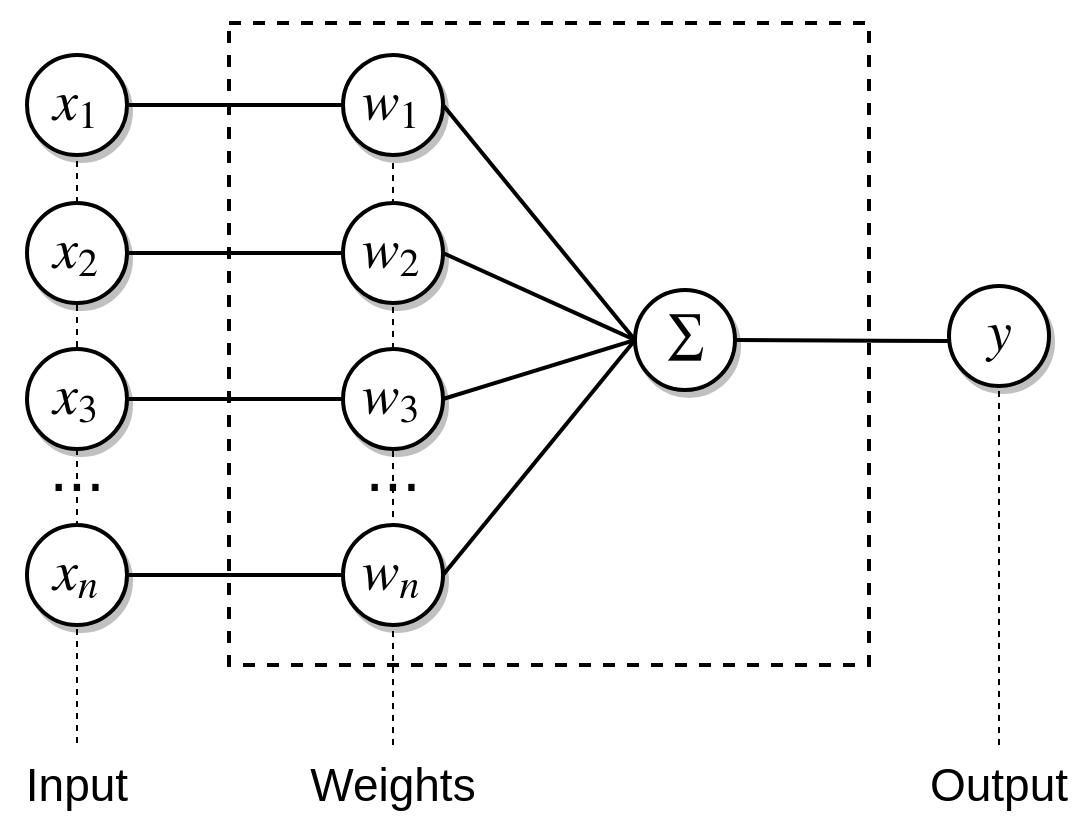
\includegraphics[width=0.6\textwidth]{pictures/perceptron}
    \centering
    \caption{graphical representation of the perceptron model.}
\end{figure}
%
ANNs are based on a fairly simple computational model called \textit{perceptron}, 
which is a transformation of an n-space into a scalar value
%
\begin{IEEEeqnarray}{rCl}
    %
    z = \sum\limits_{i = 1}^{n} (w_i \cdot x_i) + b
    %
\end{IEEEeqnarray}
%
where $x = (x_1, ..., x_n)$ is the $n$-dimensional input to the model, 
$w  = (w_1, ..., w_n)$ is a set of weights associated to each component of the 
input and $b$ is a bias term (in some notations the bias is embedded in the 
transformation by setting $x_0 = 1$ and $w_0 = b$).

In ANNs, the simple model of the perceptron is used to create a layered 
structure, in which each \textit{hidden} layer is composed by a given number 
of perceptrons (called \textit{neurons}) which:
%
\begin{enumerate}
    %
    \item take as input the output of the previous layer;
    \item are followed by a nonlinearity $\sigma$ called the \textit{activation
    function};
    \item output their value as a component of some $m$-dimensional space 
    which is the input space of the following layer.
    %
\end{enumerate}
%
\begin{figure}[h]
    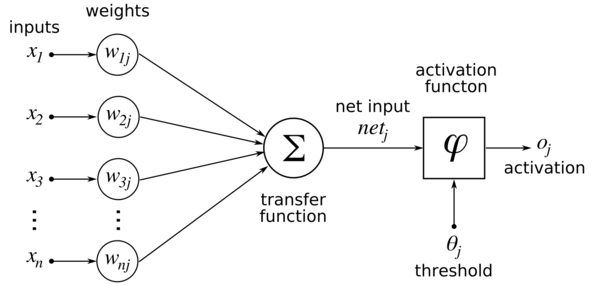
\includegraphics[width=0.6\textwidth]{pictures/neuron}
    \centering
    \caption{graphical representation of a neuron.}
\end{figure}
%
In simpler terms, each hidden layer computes an affine transformation of its 
input space:
%
    \begin{IEEEeqnarray}{rCl}
	%
	z^{(i)} = W^{(i)} \cdot \sigma(z^{(i-1)}) + B^{(i)}
	%
    \end{IEEEeqnarray}
%
where $W^{(i)}$ is the composition of the weights associated to each neuron in 
the layer and $B$ is the equivalent composition of the biases. 

The processing of the input space performed by the succession of layers which 
compose an ANN is equivalent to the composition of multiple non-linear 
transformations, which results in the production of an output vector on the 
co-domain of the target function.
%
\begin{figure}[h]
    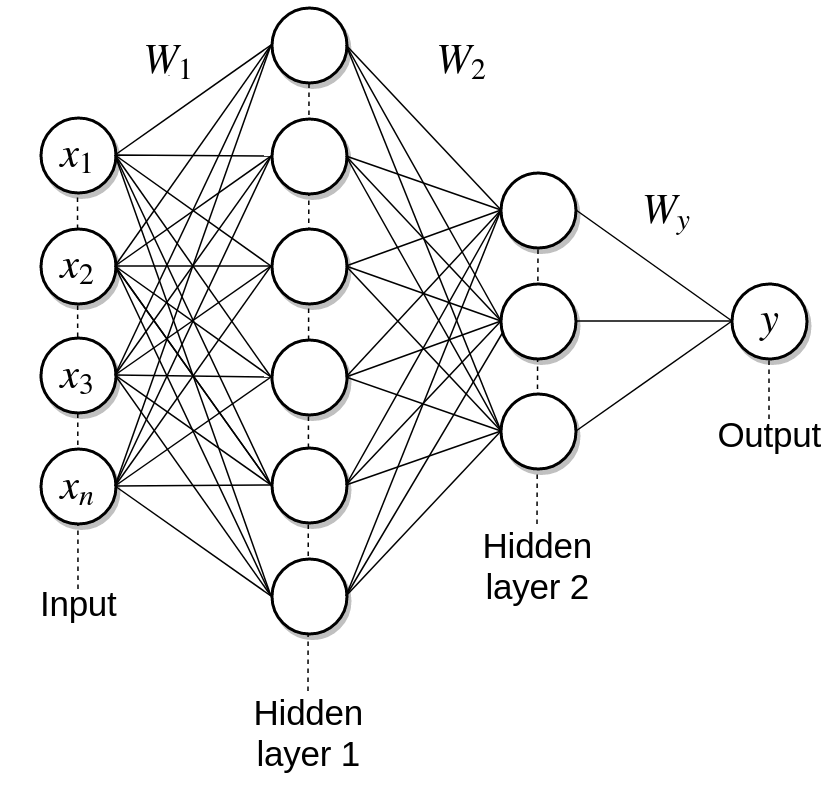
\includegraphics[width=0.6\textwidth]{pictures/ann}
    \centering
    \caption{a neural network with one hidden layer.}
\end{figure}
%

\subsection{Backpropagation}
Training ANNs is a parametric learning problem, where a \textit{loss} function 
is minimized starting from a collection of \textit{training samples} collected 
by the real process which is being approximated. In parametric learning the goal
is to find the optimal parameters of a mathematical model, such that the 
expected error made by the model on the training samples is minimized.
In ANNs, the parameters which are optimized are the weight matrices $W^{(i)}$ 
and biases $B^{(i)}$ associated to each hidden layer of the network. 

In the simple perceptron model, which basically computes a linear transformation
of the input, the optimal parameters are learned from the training set according
to the following \textit{update rule}:
%
\begin{IEEEeqnarray}{rCl}
    %
    w_i^{new} = w_i^{old} - \eta(\hat y -y) x_i, \forall i=(1, ..., n)
    %
\end{IEEEeqnarray}
%
where $\hat y$ is the output of the perceptron, $y$ is the real target from the
training set, $x_i$ is the $i$-th component of the input, and $\eta$ is a 
scaling factor called the \textit{learning rate} which regulates how much the 
weights are allowed to change in a single update. 
Successive applications of the update rule for the perceptron guarantee 
convergence to an optimum if and only if the approximated function is linear 
(in the case of regression) or the problem is linearly separable (in the case 
of classification).
%
\begin{figure}[h]
    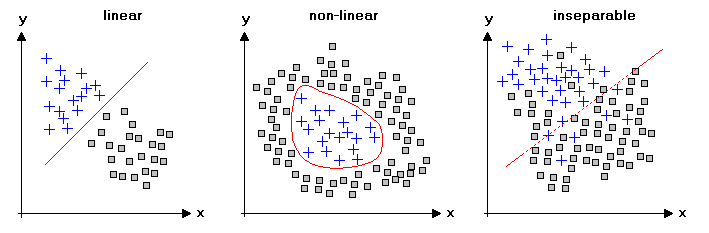
\includegraphics[width=\textwidth]{pictures/perceptron_separability}
    \centering
    \caption{different 2D classification problems, respectively linearly, 
	     non-linearly and non separable. The perceptron would be able to 
	     converge and correctly classify the points only in the first 
	     setting.}
\end{figure}
%

The simple update rule of the perceptron, however, cannot be used to train an ANN 
with multiple layers because the true outputs of the hidden layers are not
known a priori. 
To solve this issue, it is sufficient to notice that the function computed by 
each layer of a network is nonlinear, but differentiable with respect to the 
layer's input (i.e. it is linear in the weights).
This simple fact allows to compute the partial derivative of the loss function
for each weight matrix in the network to, in a sense, impute the error committed
on a training sample proportionally across neurons. The error is therefore 
propagated backwards (hence the name \textit{backpropagation}) to update all 
weights in a similar fashion to the perceptron update. 
The gradient of the loss function is then used to change the value of the 
weights, with a technique called \textit{gradient descent} which consists in 
the following update rule:
%
\begin{IEEEeqnarray}{rCl}
    %
    W_i^{new} = W_i^{old} - \eta \frac{\partial L(y, \hat y)}{\partial W_i^{old}}
    %
\end{IEEEeqnarray}
%
where $L$ is any differentiable function of the target and predicted values 
that quantifies the error made by the model on the training samples. The term 
\textit{gradient descent} is due to the fact that the weights are updated in
the opposite direction of the loss gradient, moving towards a set of parameters 
for which the loss is lower.
%
\begin{figure}[h]
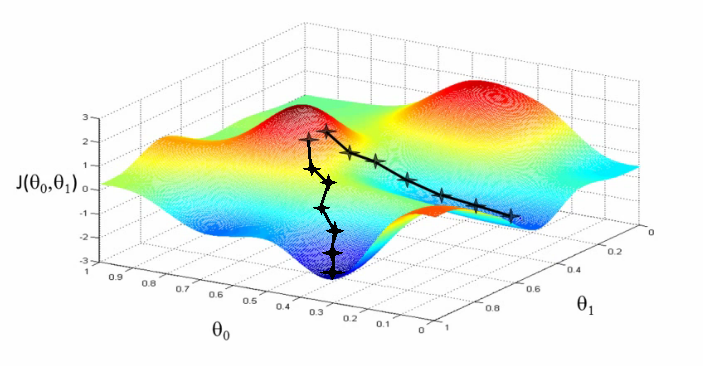
\includegraphics[width=0.8\textwidth]{pictures/SGD}
\centering
\caption{visualization of SGD on a space of two parameters.}
\end{figure}
%

Notice that traditional gradient descent optimizes the loss function over all 
the training set at once, performing a single update of the parameters. 
This approach, however, can be computationally expensive when the training set
is big; a more common approach is to use \textit{stochastic gradient descent} 
(SGD) \cite{bishop2006pattern}, which instead performs sequential parameters 
updates using small subsets of the training samples (called \textit{batches}). 
As the number of samples in a batch decreases, the variance of the 
updates increases, because the error committed by the model on a single sample 
can have more impact on the gradient step. This can cause the optimization algorithm 
to \textit{miss} a good local optima due to excessively big steps, but at the
same time could help leaving a poor local minima in which the optimization is
stuck. The same applies to the learning rate, which is the other important 
factor in controlling the size of the gradient step: if the learning rate is 
too big, SGD can \textit{overshoot} local minima and fail to converge, but at
the same time it may take longer to find the optimum if the learning rate is 
too small.
%
\begin{figure}[h]
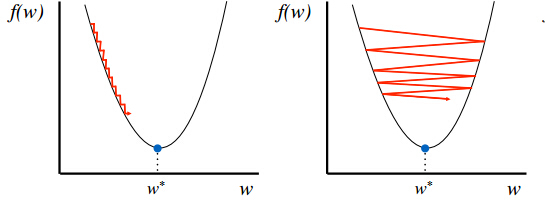
\includegraphics[width=0.6\textwidth]{pictures/SGD_overshooting}
\centering
\caption{effect of the learning rate on SGD updates. Too small (left) may 
	 take longer to converge, too big (right) may \textit{overshoot} the
	 optimum and even diverge.}
\end{figure}
%

In order to improve the accuracy and speed of SGD, some additional tweaks are
usually added to the optimization algorithm. Among these, we find the addition
of a \textit{momentum} term to the update step of SGD, in order to avoid 
oscillating in irrelevant directions by incorporating a fraction of the previous
update term in the current one:
%
\begin{IEEEeqnarray}{rCl}
    %
    W_i^{(j+1)} = W_i^{(j)} - \gamma \eta \frac{\partial L(y^{(j-1)}, \hat y^{(j-1)})}{\partial W_i^{(j-1)}} - \eta \frac{\partial L(y^{(j)}, \hat y^{(j)})}{\partial W_i^{(j)}}
    %
\end{IEEEeqnarray}
%
where $(j)$ is the number of updates that have occurred so far. In this approach, 
momentum has the same meaning as in physics, like when a body falling
down a slope tends to preserve part of its previous velocity when subjected
to a force. 
Other techniques to improve convergence include the use of an adaptive 
learning rate based on the previous gradients computed for the weights (namely
the \textit{Adagrad} \cite{duchi2011adaptive} and \textit{Adadelta} 
\cite{zeiler2012adadelta} optimization algorithms), and a similar approach 
which uses an adaptive momentum term (called \textit{Adam} \cite{kingma2014adam}).

\subsection{Convolutional Neural Networks} \label{s:CNN}
\textit{Convolutional Neural Networks} (CNNs) are a type of ANN inspired by the 
visual cortex in animal brains, and have been widely used in recent literature 
to reach state-of-the-art results in fields like computer vision, machine 
translation, and, as we will see in later sections, reinforcement learning.

CNNs exploit spatially-local correlations in the neurons of adjacent 
layers by using a \textit{receptive field}, a set of weights which is used to 
transform a local subset of the input neurons of a layer.
The receptive field is applied as a \textit{filter} over different locations of 
the input, in a fashion that resembles how a signal is \textit{strided} across 
the other during convolution. 
The result of this operation is a nonlinear transformation of 
the input space into a new space (of compatible dimensions) which preserves
the spatial information encoded in the input (e.g. form the $n \times m$ pixels
of a grayscale image to a $j \times k$ matrix that represents subgroups of 
pixels in which there is an edge).
%
\begin{figure}[h]
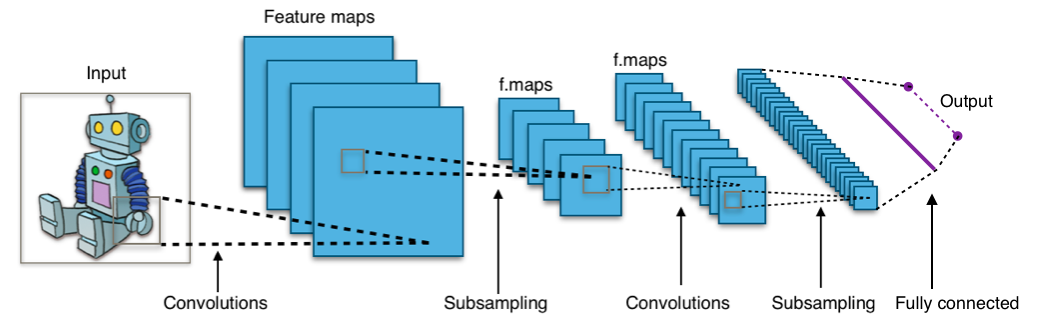
\includegraphics[width=	\textwidth]{pictures/CNN}
\centering
\caption{typical structure of a deep convolutional neural network for image
	 processing, with two convolutional hidden layers and a dense section
	 at the end (for classification or regression).}
\end{figure}
%

While standard ANNs have a \textit{fully connected} (sometimes also called 
\textit{dense}) structure, with each neuron of a layer connected to each neuron 
of the previous and following layer, in CNNs the weights are associated to a 
filter and \textit{shared} across all neurons of a layer. 
This \textit{weights sharing} has the double advantage of greatly reducing the 
number of parameters that must be updated during training, and of forcing the 
network to learn general abstractions of the input that can be applied to any 
subset of neurons covered by the filter.
%
\begin{figure}[h]
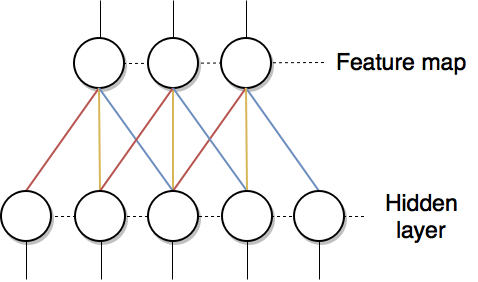
\includegraphics[width=0.5\textwidth]{pictures/shared_weights}
\centering
\caption{simple representation of shared weights in a 1D CNN. Each neuron in 
	 the second layer applies the same receptive field of three weights
	 to three adjacent neurons of the previous layer. The filter is applied 
	 with a stride of one element to produce the feature map.}
\end{figure}
%

In general, the application of a filter is not limited to one per layer and it 
is customary to have more than one filter applied to the same input in parallel,
to create a set of independent abstractions called \textit{feature maps} (also
referred to as \textit{channels}, to recall the terminology of RGB images for 
which a 3-channel representation is used for red, green, and blue). In 
this case, there will be a set of shared weights for each filter.
When a set of feature maps is given as input to a convolutional layer, a 
multidimensional filter is strided simultaneously across all channels.

At the same time, while it may be useful to have parallel abstractions of the 
input space (which effectively enlarges the output space of the layers), it is
also necessary to force a reduction of the input in order to learn useful 
representations. 
For this reason, convolutional layers in CNNs are often paired with 
\textit{pooling layers} which reduce the dimensionality of their input according
to some criteria applied to subregions of the input neurons (e.g. for each two 
by two square of input neurons, keep only the maximum activation value).
%
\begin{figure}[h]
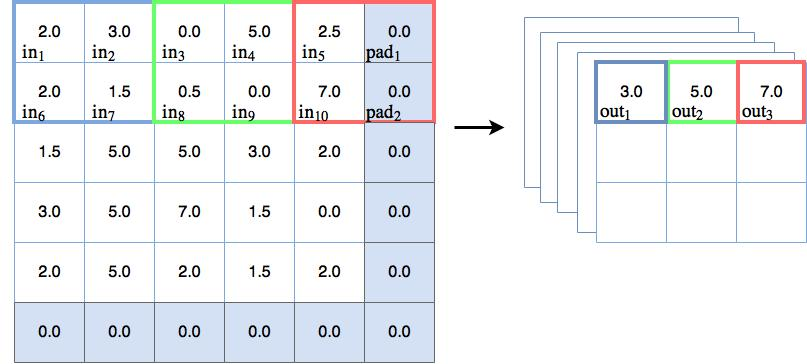
\includegraphics[width=0.7\textwidth]{pictures/max-pooling}
\centering
\caption{example of \textit{max pooling}, where only the highest activation 
	 value in the pooling window is kept.}
\end{figure}
%

Finally, typical applications of CNNs in the literature use mixed 
architectures composed of both convolutional and fully connected layers.
In tasks like image classification \cite{simonyan2014vggnet, szegedy2015going}, 
convolutional layers are used to extract significant features directly from the 
images, and dense layers are used as a final classification model; the training 
in this case is done in an end-to-end fashion, with the classification error 
being propagated across all layers to \textit{fine-tune} all weights and filters
to the specific problem.

\subsection{Autoencoders}
Autoencoders (AE) are a type of ANN which is used to learn a sparse and 
compressed representation of the input space, by sequentially compressing and 
reconstructing the inputs under some sparsity constraint.

The typical structure of an AE is split into two sections: an 
\textit{encoder} and a \textit{decoder}. In the classic architecture of 
autoencoders these two components are exact mirrors of one another, but in 
general the only constraint that is needed to define an AE is that
the dimensionality of the input be the same as the dimensionality of the output.
In general, however, the last layer of the encoder should output a reduced 
representation of the input which contains enough information for the decoder to
invert the transformation.
%
\begin{figure}[h]
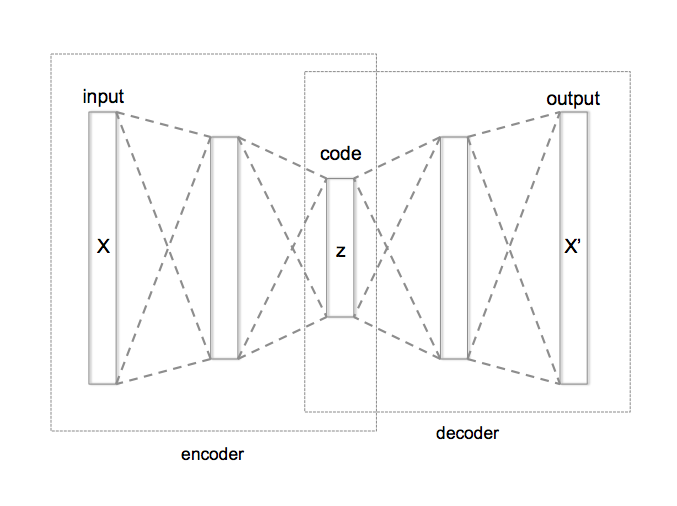
\includegraphics[width=0.7\textwidth]{pictures/autoencoder}
\centering
\caption{schematic view of an autoencoder, with the two main components 
	 highlighted.}
\end{figure}
%

The training of an AE is done in an unsupervised fashion, with no
explicit target required as the network is simply trained to predict its input.
Moreover, a strong regularization constraint is often imposed on the innermost 
layer to ensure that the learned representation is as abstract as possible 
(typically the $L1$ norm of the activations is minimized as additional term to
 the loss, to enforce sparsity). 

Autoencoders can be especially effective in extracting meaningful
features from the input space, without tailoring the features to a specific 
problem like in the end-to-end image classification example of Section 
\ref{s:CNN} \cite{erhan2010does}. 
An example of this is the extraction of features from images, 
where convolutional layers are used in the encoder to obtain an abstract 
description of the image's structure. In this case, the decoder uses
convolutional layers to transform subregions of the representation, but the 
expansion of the compressed feature space is delegated to \textit{upscaling 
layers} (the opposite of pooling layers) \cite{masci2011cae}.
This approach in building the decoder, however, can sometimes cause blurry
or inaccurate reconstructions due to the upscaling operation which simply 
replicates information rather than transforming it (like pooling layers do).
Because of this, a more sophisticated technique has been developed recently 
which allows to build purely convolutional autoencoders, without the need of 
upscaling layers in the decoder.
The layers used in this approach are called \textit{deconvolutional}\footnote{Or
\textit{transposed convolutions}.} and are thoroughly presented in 
\cite{zeiler2010deconvolutional}. For the purpose of this thesis it suffices to 
notice that image reconstruction with this type of layer is incredibly more 
accurate, down to pixel-level accuracy.

\section{Reinforcement Learning} \label{s:RL}
\textit{Reinforcement Learning} (RL) is an area of machine learning which
studies how to optimize the behavior of an agent in an environment,
in order to maximize the cumulative sum of a scalar signal called 
\textit{reward} in a setting of \textit{sequential decision making}.
RL has its roots in optimization and control theory but, because of the generality 
of its characteristic techniques, it has been applied to a variety of scientific 
fields where the concept of \textit{optimal behavior in an environment} can be 
applied (examples include game theory, multi-agent systems and economy).
The core aspect of reinforcement learning problems is to represent the setting
of an agent performing decisions in an environment, which is in turn affected by
the decisions; a scalar reward signal represents a time-discrete indicator of 
the agent's performance. This kind of setting is inspired to the natural 
behavior of animals in their habitat, and the techniques used in reinforcement 
learning are well suitable to describe, at least partially, the complexity of
living beings. 

In this section we introduce the basic setting of RL and go over a brief 
selection of the main techniques used to solve RL problems. 
%
\begin{figure}[h]
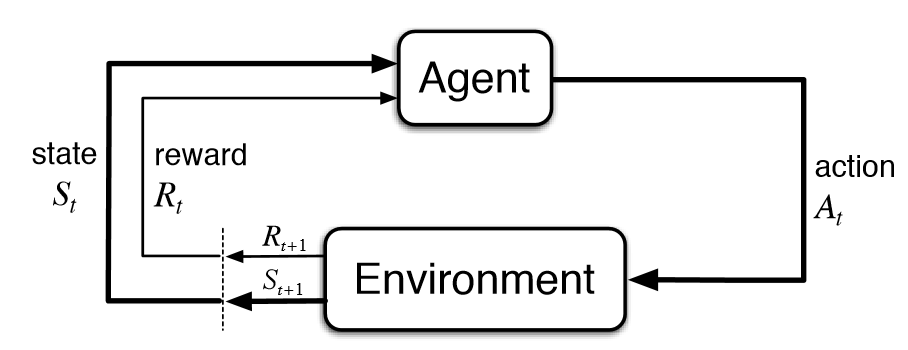
\includegraphics[width=0.7\textwidth]{pictures/reinforcement}
\centering
\caption{the reinforcement learning setting, with the agent performing actions
	 on the environment and in turn observing the state and reward.}
\end{figure}
%

\subsection{Markov Decision Processes}
\textit{Markov Decision Processes} (MDPs) are discrete-time, stochastic control 
processes, that can be used to describe the interaction of an \textit{agent} 
with an \textit{environment}.

Formally, MDPs are defined as 7-tuples $<S, S^{T}, A, P, R, \gamma, \mu>$, 
where:
\begin{itemize}
    %
    \item $S$ is the set of observable states of the environment.
    When the set if observable states coincides with the true set of states of the 
    environment, the MDP is said to be \textit{fully observable}. We will only 
    deal with fully observable MDPs without considering the case of 
    \textit{partially observable} MDPs.

    \item $S^{T} \subseteq S$ is the set of \textit{terminal states} of the 
    environment, meaning those states in which the interaction between the agent
    and the environment ends. The sequence of events that occur from when the
    agent observes an initial state until it reaches a terminal state is 
    usually called \textit{episode}.
 
    \item $A$ is the set of actions that the agent can execute in the 
    environment.
 
    \item $P: S \times A \times S \rightarrow [0,1]$ is a \textit{state 
    transition function} which, given two states $s, s' \in S$ and an action 
    $a \in A$, represents the probability of the agent going to state $s'$ by 
    executing $a$ in $s$.
 
    \item $R: S \times A \rightarrow \mathbb{R}$ is a \textit{reward function} 
    which represents the reward that the agent collects by executing an action 
    in a state. 
    
    \item $\gamma \in [0,1]$ is a \textit{discount factor} which is used to 
    weight the importance of rewards during time: $\gamma = 0$ means that only
    the immediate reward is considered, $\gamma = 1$ means that all rewards have
    the same importance.
    
    \item $\mu: S \rightarrow [0, 1]$ is a probability distribution over $S$ 
    which models the probability of starting the exploration of the environment 
    in a given state.
    %
\end{itemize}
%
\begin{figure}[h]
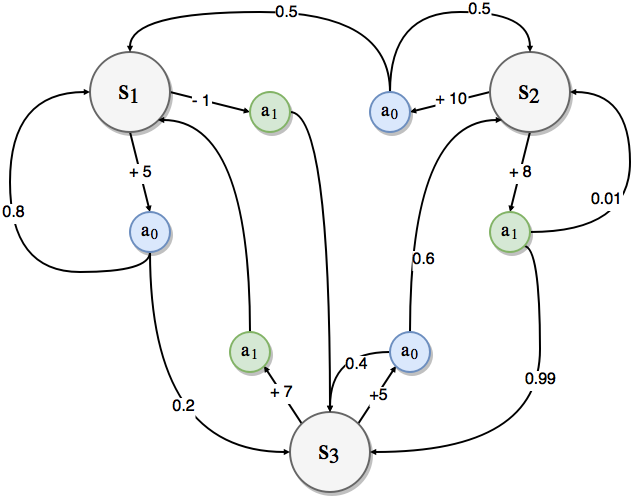
\includegraphics[width=0.5\textwidth]{pictures/mdp}
\centering
\caption{graph representation of an MDP. Each node represents a state, each arc
	 is a transition from a state to another; note that actions may have 
	 probability distributions associated to the following states.}
\end{figure}
%

Episodes are usually represented as sequences of tuples 
\[
    [(s_0, a_0, r_1, s_1), ..., (s_{n-1}, a_{n-1}, r_n, s_n)]
\]
called \textit{trajectories}, where $s_n \in S^T$, and $(s_i, a_i, r_{i+1}, s_{i+1})$ 
represents a transition of the agent to state $s_{i+1}$ by taking action $a_i$ 
in $s_i$ and collecting a reward $r_{i+1}$.

In MDPs the modeled environment must satisfy the \textit{Markov property}, 
meaning that the reward and transition functions of the environment must only 
depend on the current state and action, and not on the past state-action 
trajectory of the agent.
In other words, an environment is said to satisfy the Markov property when its 
one-step dynamics allow to predict the next state and reward given only the 
current state and action.

\subsubsection{Policy}
The behavior of the agent in an MDP can be defined as a probability 
distribution $\pi: S \times A \rightarrow [0,1]$ called a \textit{policy}, 
which given $s \in S, a \in A$, represents the probability of selecting $a$ as 
next action from $s$.
An agent which uses this probability distribution to select its next action 
when in a given state is said to be \textit{following} the policy.

A common problem when defining policies is the \textit{exploration-exploitation}
dilemma. An agent following a policy may end up observing the same trajectories 
in all episodes (e.g., when following a deterministic policy in a deterministic 
MDP), but there may be cases in which a better behavior could be had if the agent
\textit{explored} other states instead of simply \textit{exploiting} its 
knowledge. 
It is therefore common to add a probabilistic element to policies (irrespectively
of their determinism, a priori), in order to explicitly control the exploration
degree of the agent. Common techniques to control the 
\textit{exploration-exploitation} tradeoff are:
%
\begin{itemize}
    \item $\varepsilon$-greedy policies: actions are selected using a given 
    policy with probability $1-\varepsilon$, and randomly the rest of the time;
    \item softmax action selection: improves on $\varepsilon$-greedy policies by 
    reducing the number of times a suboptimal action is randomly selected. To do
    so, a probability distribution (commonly a \textit{Boltzmann distribution}) 
    dependent on the expected return from the successor states (something called
    the \textit{value} of the states, which is introduced in the next Subsection)
    is used.
\end{itemize}
%
\subsubsection{Value Functions}
Starting from the concept of policy, we can now introduce a function that 
evaluates how good it is for an agent following a policy $\pi$ to be in a given 
state. This evaluation is expressed in terms of the expected return, i.e.
the expected discounted sum of future rewards collected by an agent starting 
from a state while following $\pi$, and the function that computes it is 
called the \textit{state-value function for policy $\pi$} (or, more commonly, 
just \textit{value function}).

Formally, the state-value function associated to a policy $\pi$ is a function 
$V^{\pi}: S \rightarrow \mathbb{R}$ defined as:
%
\begin{IEEEeqnarray}{rCl}
    % Sutton, Barto
    V^{\pi}(s) & = & E_\pi[R_t | s_t = s] \\
    & = & E_\pi[\sum\limits_{k = 0}^{\infty} \gamma^k r_{t+k+1} | s_t = s]
    %
\end{IEEEeqnarray}
%
where $E_\pi[\cdot]$ is the expected value given that the agent follows 
policy $\pi$, and $t$ is any time step of an episode $[s_0, ..., s_t, ..., s_n]$
where $s_t \in S, \forall t = 0, ..., n$.

Similarly, we can also introduce a function that evaluates the goodness of 
taking a specific action in a given state, namely the expected reward obtained 
by taking an action $a \in A$ in a state $s \in S$ and then following policy 
$\pi$. 
We call this function the \textit{action-value function for policy $\pi$} 
denoted $Q^{\pi}: S \times A \rightarrow \mathbb{R}$, and defined as: 
%
\begin{IEEEeqnarray}{rCl}
    % Sutton, Barto
    Q^{\pi}(s, a) & = & E_\pi[R_t | s_t = s, a_t = a] \\
    & = & E_\pi[\sum\limits_{k = 0}^{\infty} \gamma^k r_{t+k+1} | s_t = s, a_t = a]
    %
\end{IEEEeqnarray}
%
The majority of reinforcement learning algorithms is based on computing (or 
estimating) value functions, which can then be used to control the behavior 
of the agent.
We also note a fundamental property of value functions, which satisfy particular 
recursive relationships like the following \textit{Bellman equation for 
$V^{\pi}$}:
%
\begin{IEEEeqnarray}{rCl}
    % Sutton, Barto
    V^{\pi}(s) & = & E_\pi[R_t | s_t = s] \nonumber\\
    & = & E_\pi[\sum\limits_{k = 0}^{\infty} \gamma^k r_{t+k+1} | s_t = s] \nonumber\\
    & = & E_\pi[r_{t+1} + \gamma \sum\limits_{k=0}^{\infty} \gamma^k r_{t+k+2} | s_t = s] \\
    & = & \sum\limits_{a \in A} \pi(s, a) \sum\limits_{s' \in S} P(s, a, s')[R(s, a) \>+ \nonumber\\
    && +\> \gamma E_\pi[\sum\limits_{k=0}^{\infty} \gamma^k r_{t+k+2} | s_{t+1} = s']] \\
    & = & \sum\limits_{a \in A} \pi(s, a) \sum\limits_{s' \in S} P(s, a, s')[R(s, a) + \gamma V^{\pi}(s')] \label{eq:BEV}
    %
\end{IEEEeqnarray}
%
Intuitively, relation \eqref{eq:BEV} decomposes the state-value function as the 
sum of the immediate reward collected from a state $s$ to a successor state 
$s'$, and the value of $s'$ itself; by considering the transition model of the 
MDP and the policy being followed, we see that the Bellman equation simply 
averages the expected return over all the possible $(s, a, r, s')$ transitions, 
by taking into account the probability that these transitions occur. 

\subsection{Optimal Value Functions}
In general terms, \textit{solving} a reinforcement learning task consists in 
finding a policy that yields a sufficiently high expected return. In the case of
MDPs with finite state and actions sets\footnote{We make this clarification for 
formality, but we do not expand the details further in this work. Refer to 
\cite{sutton1998reinforcement} for more details on the subjet of non-finite MDPs.}, 
it is possible to define the concept of \textit{optimal policy} as the policy 
which maximizes the expected return collected by the agent in an episode.

We start by noticing that state-value functions define a partial ordering over 
policies as follows: 
\[
    \pi \ge \pi' \iff V^{\pi}(s) \ge V^{\pi'}(s), \forall s \in S
\]
From this, the \textit{optimal policy $\pi^*$} of an MDP is a policy which is
better or equal than all other policies in the policy space. It has also been 
proven that among all optimal policies for an MDP, there is always a 
deterministic one (see Section \ref{s:value_based_optimization}).

The state-value function associated to $\pi^*$ is called the 
\textit{optimal state-value function}, denoted $V^*$ and defined as:
%
\begin{IEEEeqnarray}{rCl}
    % Sutton, Barto
    V^*(s) = \max_{\pi} V^\pi(s), \forall s \in S
    %
\end{IEEEeqnarray}
%
As we did when introducing the value functions, given an optimal policy for the 
MDP it is also possible to define the \textit{optimal action-value function} 
denoted $Q^*$:
%
\begin{IEEEeqnarray}{rCl}
    % Sutton, Barto
    Q^*(s, a) & = & \max_{\pi} Q^\pi(s, a) \\
    & = & E[r_{t+1} + \gamma V^*(s_{t+1}) | s_t = s, a_t = a] \label{eq:Qstar_V}
    %
\end{IEEEeqnarray}
%
Notice that equivalence \eqref{eq:Qstar_V} in this definition highlights the 
relation between $Q^*$ and $V^*$.

Since $V^*$ and $Q^*$ are value functions of an MDP, they must satisfy the same
type of recursive relations that we described in \eqref{eq:BEV}, in this case
called the \textit{Bellman optimality equations}.
The Bellman optimality equation for $V^*$ expresses the fact that the value of
a state associated to an optimal policy must be the expected return of the best
action that the agent can take in that state:
%
\begin{IEEEeqnarray}{rCl}
    % Sutton, Barto
    V^*(s) & = & \max_a Q^*(s, a) \label{eq:BOEV}\\
    & = & \max_a E_{\pi^*}[R_t | s_t = s, a_t = a] \\
    & = & \max_a E_{\pi^*}[\sum\limits_{k=0}^{\infty} \gamma^k r_{t+k+1}| s_t = s, a_t = a] \\
    & = & \max_a E_{\pi^*}[r_{t+1} + \gamma \sum\limits_{k=0}^{\infty} \gamma^k r_t+k+2 | s_t = s, a_t = a] \\
    & = & \max_a E_{\pi^*}[r_{t+1} + \gamma V^*(s_{t+1}) | s_t = s, a_t = a] \\
    & = & \max_a \sum\limits_{s' \in S} P(s, a, s') [ R(s, a) + \gamma V^*(s') ]
    %
\end{IEEEeqnarray}
%
The Bellman optimality equation for $Q^*$ is again obtained from the definition
as:
%
\begin{IEEEeqnarray}{rCl}
    % Sutton, Barto
    Q^*(s, a) & = & E[ r_{t+1} + \gamma \max_{a'} Q^*(s_{t+1}, a') | |s_t = s, a_t = a] \\
    & = & \sum\limits_{s'} P(s, a, s') [ R(s, a) + \gamma \max_{a'}Q^*(s', a') ]
    %
\end{IEEEeqnarray}
%
Notice that both Bellman optimality equations have a unique solution independent 
of the policy. 
If the dynamics of the environment ($R$ and $P$) are fully known, it is possible
to solve the system of equations associated to the value functions (i.e. one
equation for each state in $S$) and get an exact value for $V^*$ and $Q^*$ in 
each state. 

\subsection{Value-based optimization} \label{s:value_based_optimization}
One of main algorithm classes for solving reinforcement learning problems
is based on searching an optimal policy for the MDP by computing either 
of the optimal value functions, and then deriving a policy based on them.
From $V^*$ or $Q^*$, it is easy to determine an optimal, deterministic policy:
\begin{itemize}
    %
    \item Given $V^*$, for each state $s \in S$ there will be an action (or 
    actions) which maximizes the Bellman optimality equation \eqref{eq:BOEV}. 
    Any policy that assigns positive probability to only this action is an 
    optimal policy.
    This approach therefore consists in performing a one-step forward search on 
    the state space to determine the best action from the current state.
    \item Given $Q^*$, the optimal policy is that which assigns positive 
    probability to the action which maximizes $Q^*(s, a)$; this approach 
    exploits the intrinsic property of the action-value function of representing 
    the \textit{quality} of actions, without performing the one-step search 
    on the successor states. 
    %
\end{itemize}

In the following sections we will describe some of the most important value-based 
approaches to RL, which will be useful in the following chapters of this thesis. 
We will not deal with equally popular methods like \textit{policy gradient} or 
\textit{actor-critic} approaches, even though they have been successfully 
applied in conjunction with DL to solve complex environments (see Section 
\ref{s:DRL} and Chapter \ref{chapter3_state_of_the_art}).

\subsection{Dynamic Programming}
The use of dynamic programming (DP) techniques to solve reinforcement learning 
problems is based on recursively applying some form of the Bellman equation, 
starting from an initial policy $\pi$ until convergence to $\pi^*$.
In this class of algorithms, we identify two main approaches: \textit{policy 
iteration} and \textit{value iteration}.

\subsubsection{Policy iteration}
%
\begin{figure}[h]
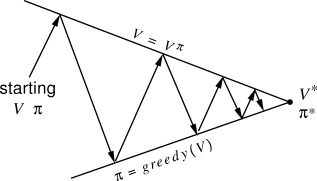
\includegraphics[width=0.5\textwidth]{pictures/policyiter}
\centering
\caption{classical representation of the policy iteration algorithm, which
	 highlights the relation between policies and their associated value
	 functions. Each pair of arrows starting from a policy and ending on a
	 greedy policy based on the value function is a step of the algorithm.}
\end{figure}
%
\textit{Policy iteration} is based of the following theorem:
\begin{theorem}[Policy improvement theorem] \label{th:pol_imp}
    % Lecture 11, slide 18
    Let $\pi$ and $\pi'$ be a pair of deterministic policies such that
    \[
        Q^\pi(s, \pi'(s)) \ge V^\pi(s), \forall s \in S 
    \]
    Then, $\pi' \ge \pi$, i.e. 
    \[
        V^{\pi'}(s) \ge V^{\pi}(s), \forall s \in S
    \]
    %
\end{theorem}

This approach works by iteratively computing the value function associated to 
the current policy, and then improving that policy by making it act greedily 
with respect to the value function, such that:
%
\begin{IEEEeqnarray}{rCl}
    % Lecture 11, slide 17
    \pi'(s) = \underset{a \in A}{\arg\max} Q^{\pi}(s, a) \label{eq:greedy_imp}
    %
\end{IEEEeqnarray}
%
For Theorem \ref{th:pol_imp}, the expected return of the policy is thus improved
because:
%
\begin{IEEEeqnarray}{rCl}	
    % Lecture 11, slide 17
    Q^\pi(s, \pi'(s)) = \max_{a \in A} Q^\pi(s, a) \ge Q^\pi(s, \pi(s)) = V^\pi(s) \label{eq:policy_improv}
\end{IEEEeqnarray}
%
This continuous improvement is applied until the inequality in \eqref{eq:policy_improv} 
becomes an equality, i.e. until the improved policy satisfies the 
Bellman optimality equation \eqref{eq:BOEV}. Since the algorithm gives no 
assurances on the number of updates required for convergence, some stopping
conditions are usually introduced to end the process when the new value function 
does not change substantially after the update (\textit{$\varepsilon$-convergence}) 
or a certain threshold number of iterations has been reached.

\subsubsection{Value iteration} \label{s:value_iteration}
Starting from a similar idea, the \textit{value iteration} approach computes 
the value function associated to an initial policy, but then applies a 
contraction operator which iterates over sequentially better value functions 
without actually computing the associated greedy policy.
The contraction operator which ensures convergence is the \textit{Bellman 
optimality backup}:
%
\begin{IEEEeqnarray}{rCl}
    % Sutton, Barto (p.266)
    V_{k+1}(s) \leftarrow \max_a \sum\limits_{s'}P(s, a, s')[R(s, a) + \gamma V(s')]
    %
\end{IEEEeqnarray}
%
As with policy iteration, convergence is ensured without guarantees on 
the number of steps, and therefore it usual to terminate the iteration according
to some stopping condition.

\subsection{Monte Carlo Methods}
Dynamic programming approaches exploit the exact solution of a value function 
which can be computed starting from a policy, but in general this requires to 
have a perfect knowledge of the environment's dynamics and may also not be 
tractable on sufficiently complex MDPs. 

\textit{Monte Carlo} (MC) methods are a way of solving reinforcement learning 
problems by only using \textit{experience}, i.e. a collection of \textit{sample 
trajectories} from an actual interaction of an agent with the environment.
This is often referred to as a \textit{model-free} approach because, while the
environment (or a simulation thereof) is still required to observe the sample
trajectories, it is not necessary to have an exact knowledge of the transition 
model and reward function of the MDP. 

Despite the differences with dynamic programming, this approach is still 
based on the same two-step process of policy iteration (evaluation and 
improvement).
To estimate the value of a state $V^\pi(s)$ under a policy $\pi$ with Monte 
Carlo methods, it is sufficient to consider a set of episodes collected under 
$\pi$: the value of the state $s$ will be computed as the average of the returns 
collected following a \textit{visit} of the agent to $s$, for all occurrences of
$s$ in the collection\footnote{Note that a variation of this 
algorithm exists, which only considers the average returns following the 
\textit{first} visit to a state in each episode.}.

This same approach can be also used to estimate the action-value function, 
simply by considering the occurrence of state-action pairs in the collected 
experience rather than states only. 

Finally, the policy is improved by computing its greedy variation \eqref{eq:greedy_imp}
with respect to the estimated value functions and the process is iteratively
repeated until convergence, with a new set of trajectories collected under each 
new policy.

\subsection{Temporal Difference Learning}
\textit{Temporal Difference} (TD) learning is an approach to RL which uses 
concepts from both dynamic programming and Monte Carlo techniques. 
TD is a \textit{model-free} approach which uses experience (like in MC)
to update an estimate of the value functions by using a previous estimate 
(like in DP).
Like MC, TD estimation uses the rewards following a visit to a state to compute
the value functions, but with two core differences:
\begin{enumerate}
    %
    \item Instead of the average of all rewards following the visit, a single 
    time step is considered (this is true for the simplest TD approach, but note 
    that in general an arbitrary number of steps can be used; the more steps are
    considered, the more the estimate is similar to the MC estimate).
    \item Estimates of the value functions are updated by using in part an 
    already computed estimate. For this reason, this approach is called a
    \textit{bootstrapping} method (like DP).
    Specifically, the iterative update step for the value function is:
    %
    \begin{IEEEeqnarray}{rCl}
	%
	V(s_t) \leftarrow V(s_t) + \alpha[r_{t+1} + \gamma V(s_{t+1}) - V(s_t)]
	%
    \end{IEEEeqnarray}
    %
    %
\end{enumerate}

In general, TD methods have several advantages over MC as they allow for an 
\textit{on-line} (i.e. they don't require full episode trajectories to work), 
bootstrapped, \textit{model-free} estimate, which is more suitable for problems 
with long or even infinite time horizons. Moreover, TD is less susceptible to 
errors or exploratory actions and in general provides a more stable learning.
It must be noted, however, that both TD and MC are guaranteed to converge given 
a sufficiently large amount of experience, and that there are problems for which 
either of the two can converge faster to the solution.

We will now present the two principal control algorithms in the TD family, one 
said to be \textit{on-policy} (i.e. methods that attempt to evaluate and improve 
the same policy that they use to make decisions) and the other 
\textit{off-policy} (i.e. methods with no relations between the estimated policy
and the policy used to collect experience).

\subsubsection{SARSA}
As usual in \textit{on-policy} approaches, \textit{SARSA}\footnote{Originally 
called \textit{on-line Q-learning} by the creators; this alternative acronym was 
proposed by Richard Sutton and reported in a footnote of the original paper in 
reference to the \textit{State, Action, Reward, next State, next Action} tuples 
which are used for prediction.} works by estimating the value $Q^\pi(s, a)$ for 
a current behavior policy $\pi$ which is used to collect sample transitions from
the environment.
The policy is updated towards greediness with respect to the estimated 
action-value after each transition $(s, a, r, s', a')$, and the action-value
is in turn updated step-wise with the following rule: 
%
\begin{IEEEeqnarray}{rCl}
    %
    Q(s_t, a_t) \leftarrow Q(s_t, a_t) + \alpha [r_{t+1} + \gamma Q(s_{t+1}, a_{t+1}) - Q(s_t,  a_t)] \label{eq:SARSA_update}
    %
\end{IEEEeqnarray}
%
The training procedure of SARSA can be summarized with Algorithm \ref{alg:SARSA}.
%
\begin{algorithm}[h]
    \caption{SARSA}
    \label{alg:SARSA}
    \begin{algorithmic}
        \STATE Initialize $Q(s,a)$ arbitrarily
        \STATE Initialize $\pi$ as some function of $Q$ (e.g. greedy)
        \REPEAT
	    \STATE Initialize $s$
	    \STATE Choose $a$ from $s$ using $\pi$
	    \REPEAT	
		\STATE Take action $a$, observe $r$, $s'$
		\STATE Choose $a'$ from $s'$ using $\pi$
		\STATE Update $Q(s, a)$ using rule \eqref{eq:SARSA_update}
		\IF{$\pi$ is time-variant}
		    \STATE Update $\pi$ towards greediness
		\ENDIF
		\STATE $s \leftarrow s'$; $a \leftarrow a'$
	    \UNTIL{$s$ is terminal or Q did not change}
	\UNTIL{training ended or Q did not change}
    \end{algorithmic}
\end{algorithm}
%

Convergence of the SARSA method is guaranteed by the dependence of $\pi$ on the
action-value function, as long as all state-action pairs are visited an infinite
number of times and the policy converges in the limit to the greedy policy (e.g. 
a time-dependent $\varepsilon$-greedy policy with $\varepsilon = 1/t$).

\subsubsection{Q-learning}
Defined by Sutton and Barto \cite{sutton1998reinforcement} as one of the most 
important breakthroughs in reinforcement learning, \textit{Q-learning} is an 
\textit{off-policy} temporal difference method that approximates the optimal 
action-value function independently of the policy being used to collect 
experiences. 
This simple, yet powerful idea guarantees convergence to the optimal 
value function as long as all state-action pairs are continuously visited (i.e. 
updated) during training.

The update rule for the TD step in Q-learning is the following: 
%
\begin{IEEEeqnarray}{rCl}
    %
    Q(s_t, a_t) \leftarrow Q(s_t, a_t) + \alpha [r_{t+1} + \gamma \max_a Q(s_{t+1}, a) - Q(s_t,  a_t)] \label{eq:QL_update}
    %
\end{IEEEeqnarray}
%
As we did for SARSA, an algorithmic description of the Q-learning algorithm is
provided in Algorithm \ref{alq:q_learning}.
%
\begin{algorithm}[h]
    \caption{Q-Learning}
    \label{alq:q_learning}
    \begin{algorithmic}
        \STATE Initialize $Q(s,a)$ and $\pi$ arbitrarily
        \REPEAT
	    \STATE Initialize $s$
	    \REPEAT	
		\STATE Choose $a$ from $s'$ using $\pi$
		\STATE Take action $a$, observe $r$, $s'$
		\STATE Update $Q(s, a)$ using rule \eqref{eq:QL_update}
		\STATE $s \leftarrow s'$
	    \UNTIL{$s$ is terminal or Q did not change}
	\UNTIL{training ended or Q did not change}
    \end{algorithmic}
\end{algorithm}
%

\subsection{Fitted Q-Iteration}
Having introduced a more classic set of traditional RL algorithms in the 
previous sections, we now present a more modern approach to solve MDPs with the 
use of supervised learning algorithms to estimate the value functions.

As we will see later in this thesis, the general idea of estimating the value 
functions with a supervised model is not an uncommon approach, and it has been 
often used in the literature to solve a wide range of environments with 
high-dimensional state-action spaces.
This approach is especially useful in problems for which the closed form solutions
of DP, or the guarantees of visiting all state-action pairs required for MC and
TD are not feasible.

Here, we choose the \textit{Fitted Q-Iteration} (FQI) approach as representative
for this whole class, because it will be used in later sections of this thesis 
as a key component of the presented methodology.
FQI is an \textit{off-line}, \textit{off-policy}, \textit{model-free}, 
\textit{value-based} reinforcement learning algorithm which computes an 
approximation of the optimal policy from a set of four-tuples $(s, a, r, s')$
collected by an agent under a policy $\pi$.
This approach is usually referred to as \textit{batch mode} reinforcement 
learning, because the complete amount of learning experience is fixed and given
a priori.

The core idea behind the algorithm is to produce a sequence of approximations of
$Q^\pi$, where each approximation is associated to one step of the 
\textit{value-iteration} algorithm seen in \ref{s:value_iteration}, and computed
using the previous approximation as part of the target for the supervised 
learning problem. The process is described in Algorithm \ref{alg:FQI}.
%
\begin{algorithm}[h]
    \caption{Fitted Q-Iteration}
    \label{alg:FQI}
    \begin{algorithmic}
        \STATE \textbf{Given}: a set $F$ of four-tuples $(s \in S, a \in A, r \in \mathbb{R}, s' \in S)$ collected with some policy $\pi$; a regression algorithm;
        \STATE $N \leftarrow 0$
        \STATE Let $\hat{Q}_N$ be a function equal to $0$ everywhere on $S \times A$
        \REPEAT
	    \STATE $N \leftarrow N+1$
	    \STATE $TS \leftarrow ((x_i, y_i), i = 0, \dots, |F|)$ such that $\forall (s_i, a_i, r_i, s'_i) \in F$:
		\begin{ALC@g}
		\STATE $x_i = (s_i, a_i)$
		\STATE $y_i = r_i + \gamma \max_{a \in A} \hat{Q}_{N-1} (s'_i, a)$
		\end{ALC@g}
	    \STATE Use the regression algorithm to induce $\hat{Q}_N(s, a)$ from $TS$
	\UNTIL{stopping condition is met}
    \end{algorithmic}
\end{algorithm}
%

Note that at the first iteration of the algorithm the action-value function is
initialized as a $0$ constant, and therefore the first approximation done by the 
algorithm is that of the reward function.
Subsequent iterations use the previously estimated function to compute the 
target of a new supervised learning problem, and therefore each step is 
independent from the previous one, except for the information of the environment 
stored in the computed approximation. 

A more practical description on how to apply this algorithm to a real problem
will be detailed in later sections of this thesis. For now, we limit this 
section to a more abstract definition of the algorithm and we do not expand 
further on the implementation details. 

\section{Deep Reinforcement Learning} \label{s:DRL}
\textit{Deep Reinforcement Learning} (DRL) is the study of reinforcement 
learning using deep neural networks as function approximators. 
The idea of combining these two areas of machine learning goes back to 
the early RL literature \cite{rummery1994line, tesauro1995temporal}, but the most
groundbreaking results were only achieved in the early 2010s, with the booming
growth in DL research that we cited in Section \ref{s:DL}.
With the advances in computing technology which enabled ANNs to be trained on 
GPUs, those RL problems which had always been characterized by an intractable 
complexity of the state space became suddenly in reach of traditional algorithms
thanks to deep learning.

Most notably, the first superhuman performance in a problem which had never 
been tackled by reinforcement learning was reached by Google DeepMind's 
\textit{Deep Q-Network} (DQN) \cite{mnih2015human}, on the \textit{Atari games} 
suite of environments. 
This introduced a new paradigm in RL, which is typical of DL approaches, of not 
performing feature engineering before feeding data to an approximator, and 
letting ANNs extract the best set of features to solve the problem from the 
raw data (in this case a sequence of frames from the games), mimicking the human
approach to problem-solving.
Other important results in DRL have been presented in recent literature, 
where convolutional neural networks were applied as approximators in classic
RL algorithms, allowing for complex state spaces (typically images of the 
environment, but also complex settings like the board in the game of \textit{Go}
) to be reduced and processed by a trainable model.

In the following section we describe the details of the above cited Deep 
Q-Network, as the most well-established DRL algorithm. We will give a wider 
overview of the state-of-the-art DRL techniques in Chapter \ref{chapter3_state_of_the_art}.

\subsection{Deep Q-Learning} \label{s:DQN}
\textit{Deep Q-learning} is an \textit{on-line}, \textit{off-policy}, 
\textit{model-free} approach to DRL.
%
\begin{figure}[h]
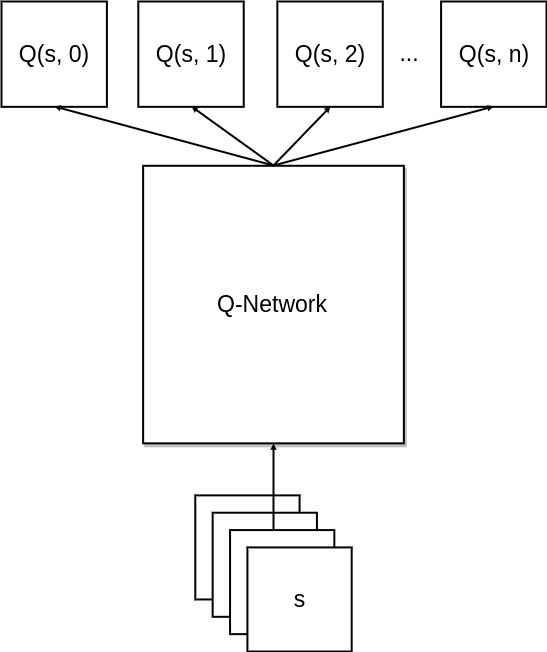
\includegraphics[width=0.4\textwidth]{pictures/dqn}
\centering
\caption{structure of the deep Q-network used by Mnih et al.\ in 
	 \cite{mnih2015human}. The network is trained to approximate the 
	 action-value function from the raw images of a game (used as states).}
\end{figure}
%
The key idea of deep Q-learning is to embed the update step of Q-learning into
the loss used for gradient descent to train a neural network (called 
\textit{deep Q-network}), resulting in the following gradient update:
%
\begin{IEEEeqnarray}{rCl}
    %
    \frac{\partial L}{\partial W_i^{old}} = E[(r + \gamma \max_{a'} Q(s', a') - Q(s, a)) \frac{\partial Q(s, a)}{\partial W_i^{old}}]
    %
\end{IEEEeqnarray}
%
The algorithm for deep Q-learning was introduced by Mnih et al. in \cite{mnih2015human}, using a
convolutional neural network with multidimensional output (one output neuron for
each action) as $Q$, and a set of samples collected with an exploratory policy 
from which the transitions for the update steps were sampled (a technique 
called \textit{experience replay}).
The CNN was structured to take as input a sequence of four frames (the states) 
from the games in the Atari suite of environments, and output an estimate of 
the action-value function which was then used to control the agent.
The samples used to update the estimates were collected with an $\varepsilon$-greedy
policy with a decaying $\varepsilon$ (hence the algorithm is \textit{off-policy}).
The algorithm proposed in the original paper is reported in Algorithm 
\ref{alg:DQL}.
%
\begin{algorithm}[h]
\caption{Deep Q-Learning with Experience Replay}
\label{alg:DQL}
    \begin{algorithmic}
	\STATE Initialize replay memory $\mathcal{D}$ to capacity $N$
	\STATE Initialize action-value function $Q$ with random weights
	\FOR{$episode = 1,M$}
	    \FOR{$t = 1,T$}
		\STATE Select a random action $a_t$ with probability $\varepsilon$
		\STATE Otherwise, select $a_t = \max_aQ^*(s_t, a)$
		\STATE Execute action $a_t$, collect reward $r_{t+1}$ and observe next state $s_{t+1}$
		\STATE Store the transition $(s_t, a_t, r_{t+1}, s_{t+1})$ in $\mathcal{D}$
		\STATE Sample random minibatch of transitions $(s_j, a_j, r_{j+1}, s_{j+1})$ from $\mathcal{D}$
		\STATE Set $ y_j = \begin{cases} r_j, & \mbox{if } s_{t+1}\mbox{ is terminal} \\ r_j + \max_{a'}Q(s_{t+1}, a'), & \mbox{otherwise}\end{cases}$
		\STATE Perform a gradient descent step using targets $y_j$
	    \ENDFOR
	\ENDFOR
    \end{algorithmic}
\end{algorithm}
%



\chapter{State Of The Art}
\label{chapter3_state_of_the_art}
\thispagestyle{empty}

\vspace{0.5cm}

The integration of RL and neural networks has a long history. Early 
RL literature \cite{rummery1994line, tesauro1995temporal, bertsekas1995neuro}
presents \textit{connectionist} approaches in conjunction with a variety
of RL algorithms, mostly using dense ANNs as approximators for the value 
functions from low-dimensional (or engineered) state spaces.
The recent and exciting achievements of DL, however, have caused a sort of RL 
renaissance, with DRL algorithms outperforming classic RL techinques on 
environments which were previously considered intractable. 
Much like the game of Chess was believed out of the reach of machines until 
IBM's Deep Blue computer \cite{campbell2002deep} won against world champion 
Garry Kasparov in 1997, DRL has paved the way to solve a wide spectrum of 
complex tasks which were previously considered a stronghold of humanity. 

In this chapter we present the most important and recent results of DRL research, 
as well as some work related to the method proposed in this thesis.

\section{Value-based Deep Reinforcement Learning} \label{SOA:value}
In 2015, Mnih et al.\ \cite{mnih2015human} introduced the \textit{deep 
Q-learning} (DQN\footnote{Acronym of \textit{Deep Q-Network.}}) algorithm which 
basically ignited the field of DRL.
The important contributions of DQN consisted in providing an end-to-end 
framework to train an agent on the \textit{Atari} environments starting from 
the pixel-level representation of the states, with a deep CNN (called 
\textit{deep Q-network}) used to estimate the $Q$ function and apply greedy 
control. The authors were able to reuse the same architecture to solve many 
different games without the need for \textit{hyperparameter tuning}, which 
proved the effectiveness of the method.

The key idea of DQN is to embed the update step of Q-learning into the loss used
for SGD to train the deep CNN, resulting in the following gradient update:
%
\begin{IEEEeqnarray}{rCl}
    %
    \frac{\partial L}{\partial W_i^{old}} = E[(r + \gamma \max_{a'} Q(s', a'; \theta') - Q(s, a)) \frac{\partial Q(s, a; \theta)}{\partial W_i^{old}}]
    %
\end{IEEEeqnarray}
%
where $\theta, \theta'$ indicate two different sets of parameters for the CNN, 
which are respectively called the \textit{online network} ($\theta$) to select 
the action for the collection of samples, and the \textit{target network} 
($\theta'$) to produce the update targets. The online network is continuously 
updated during training, whereas the target network is kept fixed for longer 
time intervals in order to stabilize the online estimate.
Moreover, a sampling procedure called \textit{experience replay} 
\cite{lin1992self} is used to stabilize training. This consists in keeping a
variable training set of transitions collected with increasingly better policies
(starting from a fully random $\varepsilon$-greedy policy and decreasing 
$\varepsilon$ as the $Q$ estimate improves), from which training samples are
randomly selected.
The full training procedure of DQN is reported in Algorithm \ref{alg:DQN}.
%
\begin{algorithm}[h]
    \caption{Deep Q-Learning with Experience Replay}
    \label{alg:DQN}
    \begin{algorithmic}
	\STATE Initialize replay memory $\mathcal{D}$ to capacity $N$
	\STATE Initialize action-value function $Q$ with two random sets of weights $\theta, \theta'$
	\FOR{$episode = 1,M$}
	    \FOR{$t = 1,T$}
		\STATE Select a random action $a_t$ with probability $\varepsilon$
		\STATE Otherwise, select $a_t = {\arg\max}_a Q(s_t, a; \theta)$
		\STATE Execute action $a_t$, collect reward $r_{t+1}$ and observe next state $s_{t+1}$
		\STATE Store the transition $(s_t, a_t, r_{t+1}, s_{t+1})$ in $\mathcal{D}$
		\STATE Sample minibatch of transitions $(s_j, a_j, r_{j+1}, s_{j+1})$ from $\mathcal{D}$
		\STATE Set $ y_j = \begin{cases} 
					r_{j+1}, & \mbox{if } s_{j+1}\mbox{ is terminal} \\ 
					r_{j+1} + \gamma \max_{a'} Q(s_{j+1}, a'; \theta'), & \mbox{otherwise}
				    \end{cases}$
		\STATE Perform a gradient descent step using targets $y_j$ with respect to the online parameters $\theta$
		\STATE Every $C$ steps, set $\theta' = \theta$
	    \ENDFOR
	\ENDFOR
    \end{algorithmic}
\end{algorithm}
%
 
From this work (which we could call introductory), many improvements have been 
proposed in the literature.
%
\begin{figure}[h]
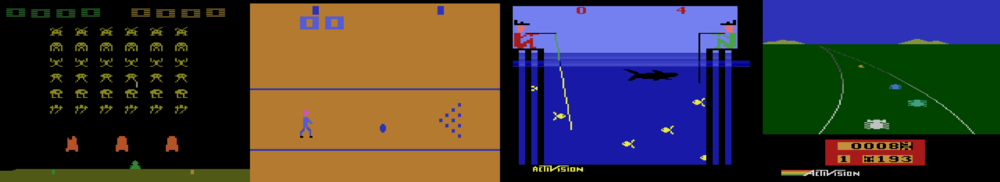
\includegraphics[width=\textwidth]{pictures/atari}
\centering
\caption{Some of the games available in the Atari environments}
\end{figure}
%
Van Hasselt et al.\ (2016) proposed \textit{Double DQN} (DDQN) \cite{van2016deep} 
to solve an over-estimation issue typical of Q-learning, due to the use of the 
maximum action value as an approximation for the maximum expected action value
(see Equation \eqref{eq:QL_update}).
This general issue was addressed by Van Hasselt (2010) with \textit{Double 
Q-learning} \cite{hasselt2010double}, a learning algorithm which keeps two 
separate estimates of the action-value function $Q^A$ and $Q^B$, and uses one to
update the other as follows:
%
\begin{IEEEeqnarray}{rCl}
    %
    Q^A(s, a) \leftarrow Q^A(s, a) + \alpha[r + \gamma Q^B(s', \underset{a}{\arg\max}Q^A(s', a)) - Q^A(s, a)]
    %
\end{IEEEeqnarray}
%
and vice-versa for $Q^B$.
DDQN uses a similar approach to limit over-estimation in DQN by evaluating the 
greedy policy according to the online network, but using the target network to 
estimate its value. This is achieved with a small change in the computation of 
the update targets:
%
\begin{IEEEeqnarray}{rCl}
    %
    y_j = \begin{cases} 
	    r_{j+1}, & \mbox{if } s_{j+1}\mbox{ is terminal} \\ 
		r_{j+1} + \gamma Q(s_{j+1}, \underset{a}{\arg\max}Q(s_{j+1}, a; \theta); \theta'), & \mbox{otherwise}
	  \end{cases}
    %
\end{IEEEeqnarray}
%    
DDQN performed better (higher median and mean score) on the 49 Atari games used 
as benchmark by Mnih et al.\ (2015), equaling or even surpassing humans on 
several games.

Schaul et al.\ (2016) \cite{schaul2016prioritized} developed the concept
of \textit{prioritized experience replay}, which replaced DQN's uniform sampling 
strategy from the replay memory with a sampling strategy weighted by the 
\textit{TD errors} committed by the network. This improved the performance of 
both DQN and DDQN.

Wang et al.\ (2016) introduced a slightly different end-to-end \textit{dueling 
architecture} \cite{wang2016dueling}, composed of two different deep estimators:
one for the state-value function $V$ and one for the \textit{advantage function} 
$A: S \times A \rightarrow \mathbb{R}$ defined as:
%
\begin{IEEEeqnarray}{rCl}
    %
    A^\pi(s, a) = Q^\pi(s, a) - V^\pi(s)
    %
\end{IEEEeqnarray}
%
In this approach, the two networks share the same convolutional layers
but use two separate dense layers. The two streams are then combined to estimate
the optimal action-value function as\footnote{In the original paper, the authors
explicitly indicate the dependence of the estimates on different 
parameters (e.g.\ $V^\pi(s, a; \phi, \alpha)$ where $\phi$ is the set of
parameters of the convolutional layers and $\alpha$ of the dense layers). 
For simplicity in the notation, here we report the estimates computed by the 
network with the same notation as the estimated functions (i.e. the network 
which approximates $V^\pi$ is indicated as $V^\pi$, and so on...).}:
%
    \begin{IEEEeqnarray}{rCl}
    %
    Q^\pi(s, a) = V^\pi(s) + (A^\pi(s, a) - \max_{a'}A^\pi(s, a'))
    %
    \end{IEEEeqnarray}
%
Several other extensions of the DQN algorithm have been proposed in recent years. 
Among these, we cite Osband et al.\ (2016) \cite{osband2016deep} who proposed 
a better exploration strategy based on Thompson sampling, to select an 
exploration policy based on the probability that it is the optimal policy; He et
al.\ (2017) \cite{he2017learning} added a constrained optimization approach 
called \textit{optimality tightening} to propagate the reward faster during 
updates and improve accuracy and convergence; Anschel et al.\ (2017) 
\cite{anschelaveraged} improved the variance and instability of DQN by averaging
previous $Q$ estimates; Munos et al.\ (2016) \cite{munos2016safe} and 
Harutyunyan et al.\ (2016) \cite{harutyunyan2016q} proposed to incorporate 
on-policy samples to the Q-learning target and seamlessly switch between 
off-policy and on-policy samples, which again resulted in faster reward 
propagation and convergence. 


\section{Other approaches}
\subsection{Memory architectures}
Graves et al.\ (2016) \cite{graves2016hybrid} proposed \textit{Differentiable 
Neural Computer} (DNC), an architecture in which an ANN has access to an 
external memory structure, and learns to read and write data by gradient descent
in a goal-oriented manner.
This approach outperformed normal ANNs and DNC's precursor \textit{Neural 
Turing Machine} \cite{gravesneural} on a variety of query-answering and natural 
language processing tasks, and was used to solve a simple \textit{moving block} 
puzzle with a form of reinforcement learning in which a sequence of instructions
describing a goal is coupled to a reward function that evaluates whether the 
goal is satisfied (a set-up that resembles an animal training protocol with a 
symbolic task cue).
%
\begin{figure}[h]
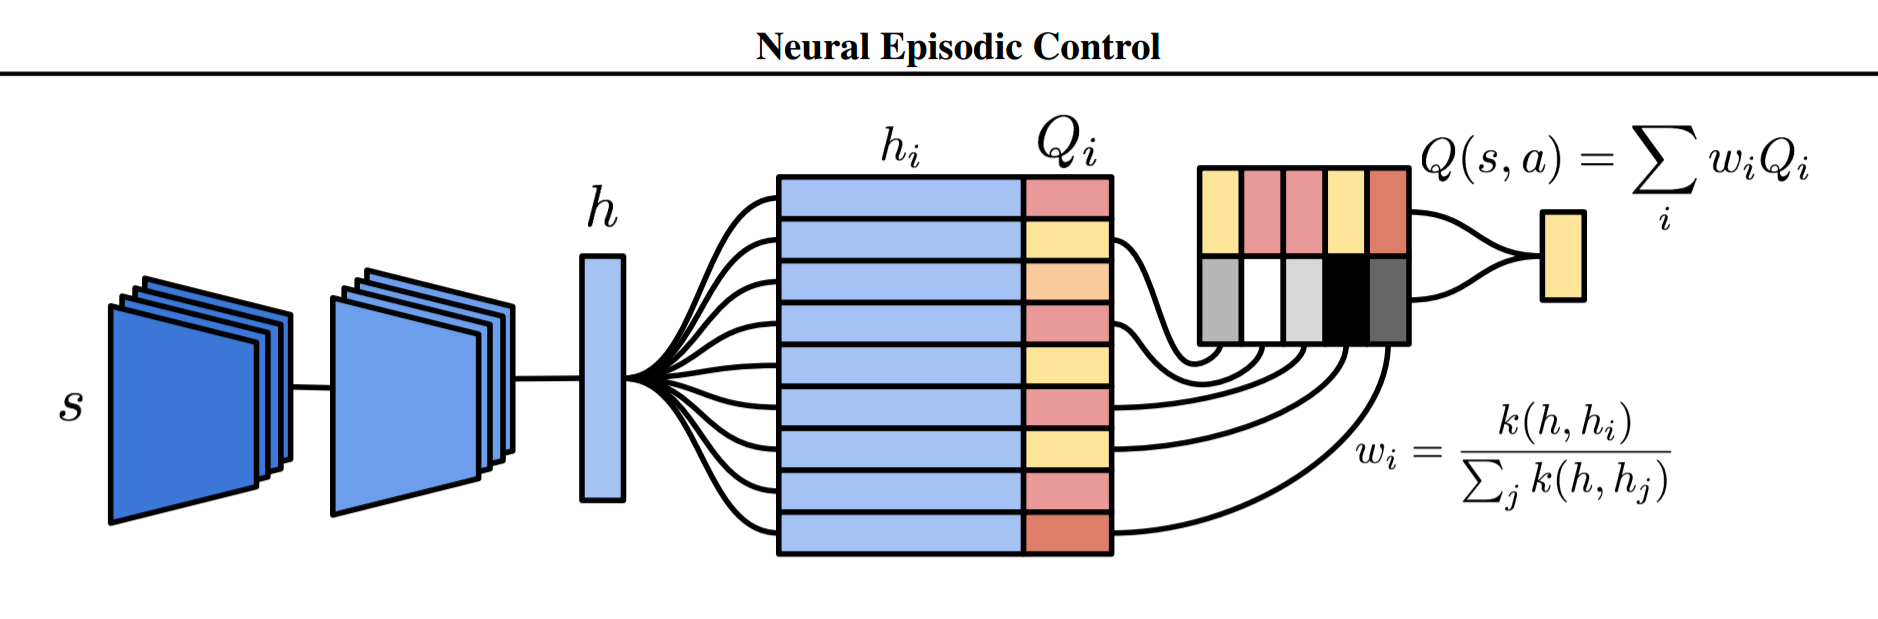
\includegraphics[width=\textwidth]{pictures/nec}
\centering
\caption{Architecture of NEC}
\label{f:nec}
\end{figure}
%

Pritzel et al.\ (2017) \cite{pritzel2017neural} extended the concept of 
differentiable memory to DQN with \textit{Neural Episodic Control} (NEC). 
In this apporach, the DRL agent consists of three components: a CNN which 
processes pixel images, a set of memory modules (one per action), and a dense 
ANN which converts read-outs from the action memories into action-values. The 
memory modules, called \textit{differentiable neural dictionaries} (DNDs), are 
memory structures which resemble the dictionary data type found in computer 
programs. DNDs are used in NEC to associate the state embeddings computed by the
CNN to a corresponding $Q$ estimate, for each visited state: a read-out for a 
key consists in a weighted sum of the values in the DND, with weights given by 
normalized kernels between the lookup key and the corresponding key in memory 
(see Figure \ref{f:nec}). 
DNDs are populated automatically by the algorithm without learning what to write,
which greatly speeds up the training time with respect to DNC.

NEC outperformed every previous DRL approach on Atari games, by achieving better
results using less training samples.

\subsection{AlphaGo}
Traditional board games like chess, checkers, Othello and Go are classical 
test benches for artificial intelligence. Since the set of rules which
characterizes this type of games is fairly simple to represent in a program, the
difficulty in solving these environments stems from the complexity of the 
state space. Among the cited games, Go was one of the last board games in which 
an algorithm had never beaten top human players, because its characteristic 
$19 \times 19$ board which allows for approximately $250^{150}$ sequences of
moves\footnote{Number of legal moves per position elevated to the length of the 
game.} was too complex for exhaustive search methods.
%
\begin{figure}[h]
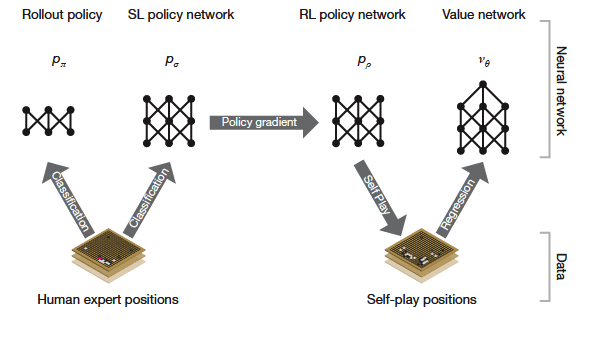
\includegraphics[width=0.7\textwidth]{pictures/alphago}
\centering
\caption{Neural network training pipeline of AlphaGo}
\label{f:alphago}
\end{figure}
%

Silver et al.\ (2016) \cite{silver2016mastering} introduced \textit{AlphaGo}, 
a computer program based on DRL which won 5 games to 0 against the European Go 
champion in October 2015; soon after that, AlphaGo defeated 18-time world 
champion Lee Sedol 4 games to 1 in March 2016, and world champion Ke Jie 3 to 0 
in May 2017. After these results, Google DeepMind (the company behind 
AlphaGo) decided to retire the program from official competitions and released a
dataset containing 50 self-play games \cite{alphago}.

AlphaGo is a complex architecture which combines deep CNNs, reinforcement 
learning, and Monte Carlo Tree Search (MCTS) \cite{browne2012survey, gelly2012grand}. 
The process is divided in two phases: a neural network training pipeline and 
MCTS. In the training pipeline, four different networks are trained: a 
\textit{supervised learning} (SL) policy network trained to predict human moves;
a \textit{fast} policy network to rapidly sample actions during MC rollouts; a 
\textit{reinforcement learning} policy network that improves the SL network by 
optimizing the final outcome of games of self-play; a \textit{value} network 
that predicts the winner of games (see Figure \ref{f:alphago}). 
Finally, the policy and value networks are combined in an MCTS algorithm that 
selects actions with a lookahead search, by building a partial search tree using
the estimates computed with each network.

\subsection{Asynchronous Advantage Actor-Critic}
\textit{Actor-critic} algorithms \cite{sutton1998reinforcement} are TD methods 
that have a separate memory structure to explicitly represent the policy 
independent of the value function. The policy structure is known as the actor, 
because it is used to select actions, and the estimated value function is known 
as the critic, because it criticizes the actions made by the actor.
%
\begin{figure}[h]
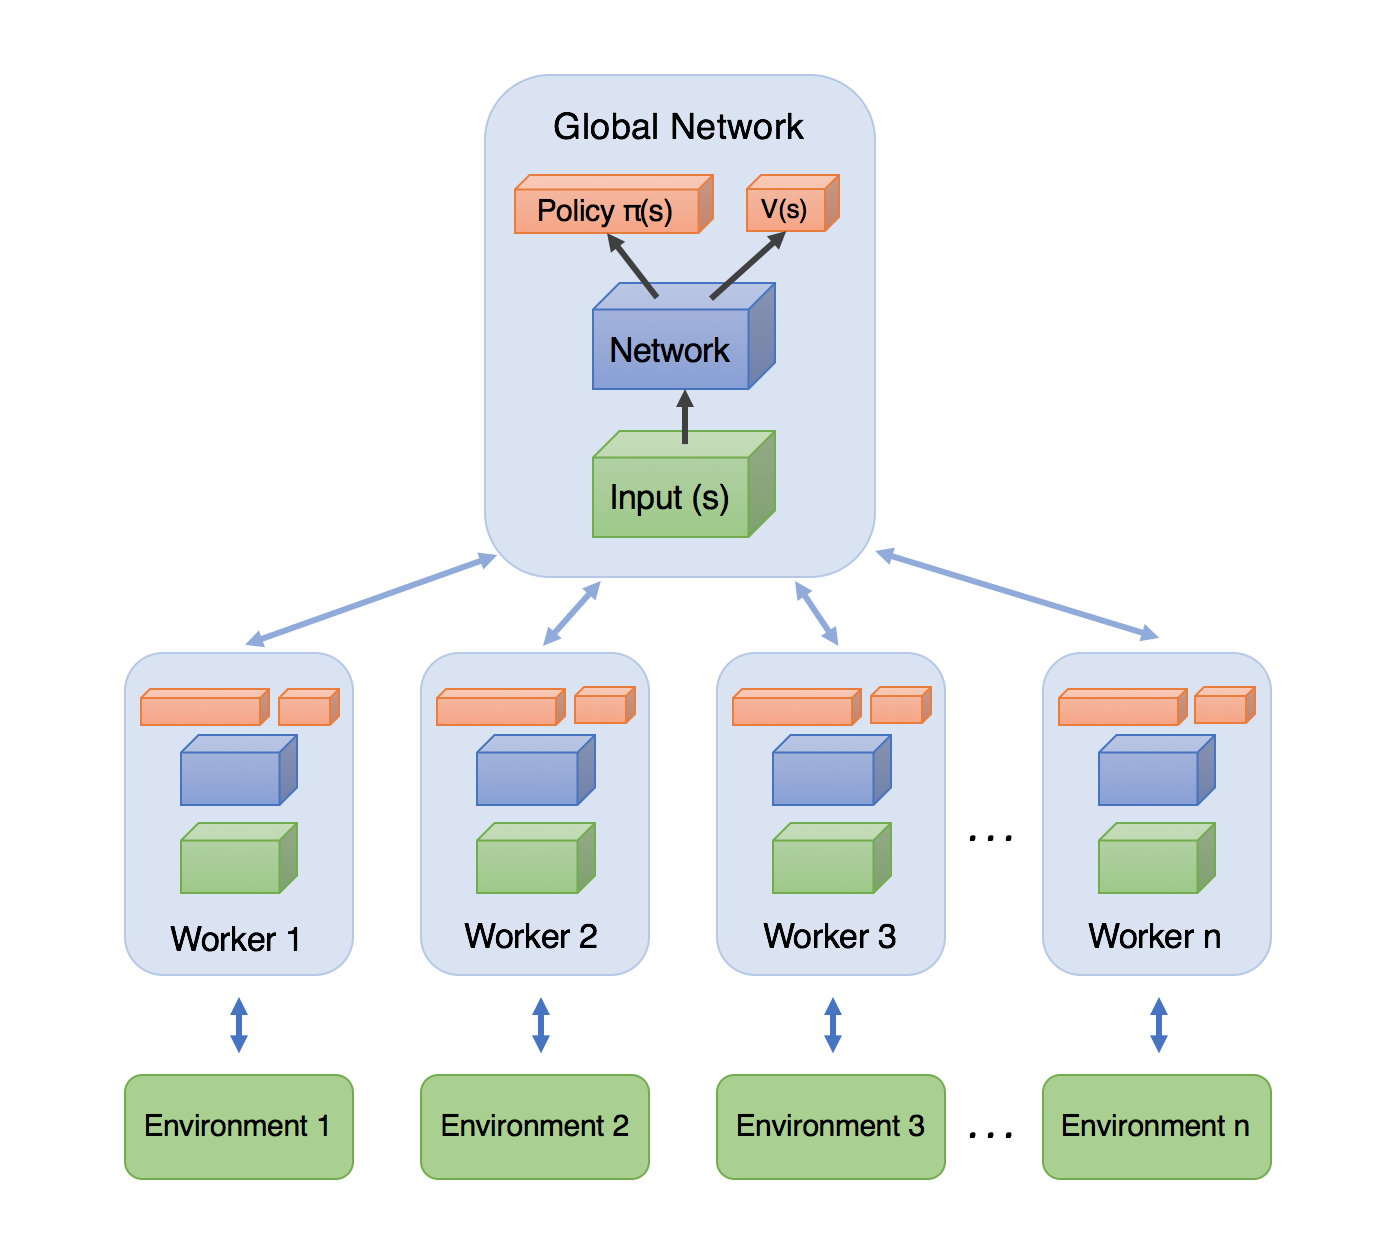
\includegraphics[width=0.5\textwidth]{pictures/a3c}
\centering
\caption{The asynchronous architecture of A3C}
\end{figure}
%
Mnih et al.\ (2016) \cite{mnih2016asynchronous} presented a deep variation of 
the actor-critic algorithm, called \textit{Asynchronous Advantage Actor-Critic} 
(A3C). In this approach, different instances of actor-critic pairs are run in 
parallel to obtain a lower-variance estimate of the value function, without the 
need of a replay memory to stabilize training. Each \textit{worker} consists in 
a deep CNN with a unique convolutional section and two separate dense networks
on top, one for the value function and one for the policy. 

This asynchronous methodology was applied to other classical RL algorithms in 
the same paper; we only report the actor-critic variant as it was the best 
performing, with notably shorter training times and performance comparable 
to DQN and its variations.

\section{Related Work}
Lange and Riedmiller (2010) \cite{lange2010deep} proposed the \textit{Deep 
Fitted Q-iteration} (DFQ) algorithm, a batch RL method which used deep dense 
autoencoders to extract a state representation from pixel images. 
In this algorithm, a training set of $(s, a, r, s')$ transitions is collected
with a random exploration strategy, where $s, s'$ are pixel images of two 
consecutive states. The samples are then used to train a dense autoencoder with 
two neurons in the innermost layer, which in turn is used to encode all states 
in the training set. This encoded dataset is then passed as input to FQI, 
which produces an estimate for the $Q$ function using a kernel based 
approximator. A new policy is then computed from the estimated $Q$ and the 
encoder, and the process is repeated starting with the new policy until the 
obtained $Q$ is considered satisfactory.
The authors applied DFQ to a simple \textit{Gridworld} environment with fixed 
size and goal state, and were able to outperform other image-based feature
extraction methods (like \textit{Principal Components Analysis} 
\cite{wold1987principal}) with good sample efficiency.

% Another work which has common aspects with our method is the one by Anderson et
% al.\ (2015) \cite{anderson2015faster}, who improved convergence of DRL on 
% simple problems (e.g.\ \textit{Cart-pole} and \textit{Dynamic cart}) by 
% pre-training the Q-network to predict state dynamics.



























\chapter{Fitted Q-Iteration with Deep State-Dynamics Features}
\label{ch3_setup}
\thispagestyle{empty}

\vspace{0.5cm}

As central argument of this thesis, we propose a DRL method which 
combines the feature extraction capabilities of deep CNNs with the quick 
and powerful batch RL approach of FQI. 
Given a high-dimensional state space of pixels representing sequences of 
greyscale frames from an Atari game, we use a deep convolutional autoencoder 
to map the original state space to a compressed \textit{feature space} which 
accounts for both the states and their one-step dynamics (i.e. the transition 
model). This compressed representation is then used to run a \textit{tree-based}
FQI algorithm in batch mode.

In this chapter we give a formal description of the method and its core 
components. Technical details of implementation will be discussed in the next
chapter.

\section{Motivation}
% TODO: remove part on dynamics1
The state-of-the-art DRL methods listed in the previous chapter are able to 
outperform classic RL algorithms in a wide variety of problems, and in some 
cases are the only possible way of dealing with high-dimensional control 
settings like the Atari games. 
However, the approaches cited above tend to be grossly 
\textit{sample-inefficient}, requiring tens of millions of samples collected
on-line to reach optimal performance. Several publications successfully deal 
with this aspect, but nonetheless leave room for improvement (lowering at most
by one order of magnitude the number of samples required).
The method introduced by Lange and Riedmiller (2010) \cite{lange2010deep} is 
similar to ours but their dense architecture predates the more modern 
convolutional approaches in image processing and is less suited for complex
tasks than our AE.

The method that we propose tries to improve both aspects of information content
of the compressed feature space and sample efficiency. We extract general 
features from the environments and try to reach better or equivalent performance
in up to two orders of magnitude less samples than DQN on Atari games.

\section{Problem Formulation}
% TODO: add RFS
The general setting of this problem is typical of DRL problems: we use a deep 
ANN to extract a representation of an environment, and use that representation 
to control an agent with standard RL algorithms. We add an additional step after
the deep feature extraction to further reduce the representation down to the 
essential bits of information required to solve the problem by using the 
\textit{Recursive Feature Selection} (RFS) algorithm \cite{castelletti2011tree}.

In our approach we use a modular architecture with three separate stages for the
training phase, and combine the three stages in an end-to-end fashion during
the control phase. The main components of the algorithm are:
%
\begin{enumerate}
    \item a deep convolutional autoencoder which we use to extract a 
    representation of the environment;
    the purpose of the AE is to map the original, pixel-level state space $S$ of
    the environment into a strongly compressed feature space ${\tilde{S}}$ which
    contains information of both the state space and part of the transition 
    model of the environment;
    \item a \textit{Recursive Feature Selection} (RFS) technique to further 
    reduce the state representation $\tilde{S}$ and keep only the truly 
    informative features extracted by the AE, effectively mapping the extracted 
    state-space to a subspace $\hat{S}$.
    \item a \textit{tree-based} FQI learning algorithm which produces an 
    estimator for the action-value function, with $\hat{S}$ as domain. 
\end{enumerate}
%
The three components are separately trained to produce the following 
transformations respectively:
\begin{itemize}
    \item $ENC: S \rightarrow \tilde{S}$, from the pixel representation to a 
    compressed feature space;
    \item $RFS: \tilde{S} \rightarrow \hat{S}$, from the compressed feature space
    to a minimal subspace with the most informative features;
    \item $\hat{Q}^\pi: \hat{S} \times A \rightarrow \mathbb{R}$, an 
    action-value function on $\hat{S}$.
\end{itemize}

After the training phase, we simply combine the three functions to obtain the 
action-value function $Q^\pi: S \times A \rightarrow \mathbb{R}$ as follows: 
%
\begin{IEEEeqnarray}{rCl}
    %
    Q^\pi(s, a) = \hat{Q}^\pi(RFS(ENC(s)), a)
    %
\end{IEEEeqnarray}
%
A general description of the process is given in Algorithm \ref{alg:FQI-DSDF}.
%
\begin{algorithm}[h]
    \caption{Fitted Q-Iterations with Deep State Features}
    \label{alg:FQI-DSDF}
    \begin{algorithmic}
	\STATE \textbf{Given}: an arbitrary policy $\pi$;
	\STATE Initialize the encoder $ENC: S \rightarrow \tilde{S}$ arbitrarily;
	\STATE Initialize the decoder $DEC: \tilde{S} \rightarrow S$ arbitrarily;
	\REPEAT 
	    \STATE Collect a set $\mathcal{TS}$ of four-tuples $(s \in S, a \in A, r \in \mathbb{R}, s' \in S)$ using $\pi$;
	    \STATE Train the composition $DEC \circ ENC: S \rightarrow S$ using the first column of $\mathcal{TS}$ as input and target;
	    \STATE Build a set $\mathcal{TS}_F$ of four-tuples $(f \in \tilde{S}, a \in A, r \in \mathbb{R}, f' \in \tilde{S})$ by applying the encoder to the first and last column of $\mathcal{TS}$ s.t. $f = ENC(s)$;
	    \STATE Call the RFS feature selection algorithm on $\mathcal{TS}_F$ to obtain a space reduction $FS: \tilde{S} \rightarrow \hat{S}$;
	    \STATE Build a set $\mathcal{TS}_{\hat{F}}$ of four-tuples $(\hat{f} \in \hat{S}, a \in A, r \in \mathbb{R}, \hat{f'} \in \hat{S})$ by applying $RFS$ to the first and last column of $\mathcal{TS}_F$ s.t. $\hat{f} = RFS(f)$;
	    \STATE Call FQI on $\mathcal{TS}_{\hat{F}}$ to produce $\hat{Q}^\pi: \hat{S} \times A \rightarrow \mathbb{R}$;
	    \STATE Combine $\hat{Q}^\pi$, $RFS$ and $ENC$ to produce $Q^\pi: S \times A \rightarrow \mathbb{R}$:
		\[
		Q^\pi(s, a) = \hat{Q}^\pi(RFS(ENC(s)), a)
		\]
	    \STATE Set $\pi(s) = \underset{a}{\arg\max} Q^{\pi}(s, a)$;
	\UNTIL{stopping condition is met;}
    \end{algorithmic}
\end{algorithm}
%
\section{Extraction of State Features}
% TODO: remove part on dynamics
The AE used in our approach consists of two main components, namely an 
\textit{encoder} and a \textit{decoder} (cf. \ref{s:AE}). To the end of 
explicitly representing the encoding purpose of the AE, we keep a separate 
notation of the two modules; we therefore refer to two different CNNs, namely 
$ENC: S \rightarrow \tilde{S}$ that maps the original state space to the 
compressed representation $\tilde{S}$, and $DEC: \tilde{S} \rightarrow S$ which
performs the inverse transformation. The full AE is the composition of the two 
networks $AE: DEC \circ ENC: S \rightarrow S$. Note that the composition is 
differentiable end-to-end, and basically consists in \textit{plugging} the last
layer of the encoder as input to the decoder. 

We train the AE to extract\footnote{By \textit{extraction} we mean the 
transformation computed by the encoder.} a joint representation of the 
environment's state and dynamics by SGD, using a training set of $(s, s')$ 
tuples of consecutive states collected with a sufficiently explorative policy. 
The AE must therefore learn to map a state to its successor under the sampling 
policy. 

This ...

\section{Tree-based Recursive Feature Selection}
% TODO

\section{Tree-based Fitted Q-Iteration}
% TODO
\chapter{Technical Details and Implementation}
\label{ch5_arch}
\thispagestyle{empty}

\vspace{0.5cm}

In this chapter we show the implementation details of the architecture
used to perform experiments. We try to provide a complete description of the 
parametrization of the components and of the training procedure to ensure 
reproducibility of the experimental results.

\section{Atari Environments}
The \textit{Arcade Learning Environment} (ALE) \cite{bellemare2013arcade} is an 
evaluation platform for RL agents.
ALE offers a programmatic interface to hundreds of game environments for the 
\textit{Atari 2600}, a popular home video game console developed in 1977 with 
more than 500 games available, and is often referred to simply as 
Atari environments (or games). 
We use the implementation of ALE provided by the \textit{Gym 0.8.1} package for 
Python 2.7, developed by OpenAI and maintained as an open source project. 
This implementation provides access to the game state in the form of 
$3 \times 110 \times 84$ RGB frames, produced at an internal frame-rate of $60$ 
frames per second (FPS).
When an action is executed in the environment, the simulator repeats the action 
for four consecutive frames of the game and then provides another observation, 
effectively lowering the frame rate from $60$ FPS to $15$ FPS and making the 
effects of actions more evident. 
We perform a preprocessing operation on the states similar to that performed
by Mnih et al.\ in DQN, in order to include all necessary information about
the environment and its nominal dynamics in the new state representation.
First we convert each RGB observation to a single-channel greyscale 
representation in the discrete 8-bit interval $[0, 255]$ using the 
\textit{ITU-R 601-2 luma transform}:
%
\begin{IEEEeqnarray}{rCl}
    %
    L = \frac{299}{1000}R + \frac{587}{1000}G + \frac{114}{1000}B
    %
\end{IEEEeqnarray}
%
where $R$, $G$, $B$ are the 8-bit components of the image. We then normalize 
these values in the $[0, 1]$ interval via \textit{max-scaling} (i.e.\ dividing 
each pixel by $255$).
We also reduce the height of the image by two pixels in order to prevent 
information loss due to a rounding operation performed by the convolution
method used in the AE.
Finally, we concatenate the preprocessed observation to the last three 
preprocessed frames observed from the environment, effectively blowing up the
state space to a $4 \times 108 \times 84$ vector space. The initial state for
an episode is artificially set as a repetition of the first observation provided
by the simulator. 
% TODO: put an image here to expalin the sampling technique.
    
Moreover, in order to facilitate comparisons and improve stability, we remain 
loyal to the methodology used for DQN and perform the same clipping of the 
reward signal in a $[-1, 1]$ interval. 

We add a final tweak to the Gym implementation of ALE in order to fix a 
requirement of some of the environments to perform some specific actions in 
order to start an episode (e.g.\ in \textit{Breakout} it is required that the 
agent takes actions 1, 4 or 5 to start the game). We automatically start each 
episode by randomly selecting one of the initial actions of the game and forcing
the agent to take that action at the beginning of the episode. 

\section{Autoencoder}
%
\begin{table}[h]
    \centering
    \begin{tabular}{l c c c c c c} 
	\hline
	Type & Input & Output & \# Filters & Filter & Stride & Activation \\ 
	\hline 
	Conv. & $4 \times 108 \times 84$ & $32 \times 26 \times 20$ & $32$ & $8 \times 8$ & $4 \times 4$ & ReLU \\ 
	Conv. & $32 \times 26 \times 20$ & $64 \times 12 \times 9$ & $64$ & $4 \times 4$ & $2 \times 2$ & ReLU \\ 
	Conv. & $64 \times 12 \times 9$ & $64 \times 10 \times 7$ & $64$ & $3 \times 3$ & $1 \times 1$ & ReLU \\ 
	Conv. & $64 \times 10 \times 7$ & $16 \times 8 \times 5$ & $16$ & $3 \times 3$ & $1 \times 1$ & ReLU \\ 
	Flatten	& $16 \times 8 \times 5$ & $640$ & - & - & - & - \\ 
	\hline
	Reshape & $640$ & $16 \times 8 \times 5$ & - & - & - & - \\
	Deconv. & $16 \times 8 \times 5$ & $16 \times 10 \times 7$ & $16$ & $3 \times 3$ & $1 \times 1$ & ReLU \\ 
	Deconv. & $16 \times 10 \times 7$ & $64 \times 12 \times 9$ & $64$ & $3 \times 3$ & $1 \times 1$ & ReLU \\
	Deconv. & $64 \times 12 \times 9$ & $64 \times 26 \times 20$ & $64$ & $4 \times 4$ & $2 \times 2$ & ReLU \\
	Deconv. & $64 \times 26 \times 20$ & $32 \times 108 \times 84$ & $32$ & $8 \times 8$ & $4 \times 4$ & ReLU \\
	Deconv. & $32 \times 108 \times 84$ & $4 \times 108 \times 84$ & $4$ & $1 \times 1$ & $1 \times 1$ & Sigmoid \\
	\hline
    \end{tabular}
    \caption{Layers of the autoencoder with key parameters}
    \label{t:AE_structure}
\end{table}
%
We structure the AE to take as input the preprocessed observations from the
environment and predict values on the same vector space.
The first four convolutional layers make up the encoder and perform a 2D 
convolution with the \textit{valid} padding algorithm such that the input of 
each layer (in the format $channels \times height \times width$) is reduced 
automatically across the last two dimensions (height and width) according to the
following formula: 
%
\begin{IEEEeqnarray}{rCl}
    %
    output_i = \lfloor(input_i - filter_i  + stride_i) / stride_i\rfloor
    %
\end{IEEEeqnarray}
%
Since the main purpose of pooling layers is to provide translation invariance to 
the representation of the CNN (meaning that slightly shifted or tilted inputs
are considered the same by the network), here we choose to not use pooling 
layers in order to preserve the precious information regarding the position of
different elements in the games; this same approach was adopted in DQN.
A final \textit{Flatten} layer is added at the end of the encoder to provide a 
1D representation of the feature space, which is reversed before the beginning 
of the decoder. 

The decoder consists of deconvolutional layers with symmetrical filter sizes, 
filter numbers and strides with respect to the encoder. Here the \textit{valid} 
padding algorithm is inversed to expand the representation with this formula:
%
\begin{IEEEeqnarray}{rCl}
    %
    output_i = \lfloor (input_i \cdot stride_i) + filter_i  - stride_i\rfloor
    %
\end{IEEEeqnarray}
% 
A final deconvolutional layer is added at the end to reduce the number of 
channels back to the original four, without changing the width and height of
the frames (i.e.\ using unitary filters and strides).
All layers in the autoencoder use the \textit{Rectified Linear Unit} (ReLU) 
\cite{nair2010rectified, krizhevsky2012imagenet} nonlinearity as activation 
function, except for the last layer which uses \textit{sigmoids} to limit the 
activations values in the same $[0, 1]$ interval of the input.
Details of the AE layers are summarized in Table \ref{t:AE_structure}.

We train the AE with the Adam optimization algorithm \cite{kingma2014adam} 
(see Table \ref{t:adam_params} for details on the hyperparameters) set to 
minimize the \textit{binary crossentropy} loss defined as:
%
\begin{IEEEeqnarray}{rCl}
    %
    L(y, \hat y) = - \frac{1}{N} \sum\limits_{n=1}^{N}[y_n log(\hat y_n) + (1-y_n) log(1-\hat y_n)]
    %
\end{IEEEeqnarray}
%
where $y$ and $\hat y$ are vectors of $N$ target and predicted observations in 
the state space. The dataset used for training is a subset of the dataset 
collected for the whole learning procedure described in Algorithm 
\ref{alg:FQI-DSDF}, namely the first and last elements of the four-tuples
$(s, a, r, s') \in \mathcal{TS}$.
%
\begin{table}[h]
    \centering
    \begin{tabular}{l c} 
	\hline
	Parameter & Value \\ 
	\hline 
	Learning rate &  $0.001$ \\
	Batch size & $32$ \\
	Exponential decay rate ($\beta_1$) & $0.9$ \\
	Exponential decay rate ($\beta_2$) & $0.999$ \\
	Fuzz factor ($\varepsilon$) & $10^{-8}$ \\
	\hline
    \end{tabular}
    \caption{Optimization hyperparameters for Adam}
    \label{t:adam_params}
\end{table}
%

We prevent \textit{overfitting} of the training set by monitoring the 
performance of the AE on a held-out set of validation samples, and stopping the 
procedure when the validation loss does not improve for five consequent 
training epochs. 

Finally, we modify the loss function to account for the sparsity of the reward
signal of the environment. Atari games produce a positive reward for the agent
only on rather rare events, such as scoring a point in \textit{Pong} or breaking
a brick in \textit{Breakout}, whereas for the majority of the time the agent
collects a null reward. This means that any training set with samples collected
by playing a game will have an unbalance between the transitions in which the 
game is in a \textit{nominal} behavior and those in which the agent collects the
reward. 
To deal with this unbalance, we introduce a weighting factor by which we scale 
the gradient associated to each sample. Since each training sample of the AE
is associated to a transition $(s_i, a_i, r_i, s'_i) \in \mathcal{TS}$, we 
compute the sample weights for $(s_i, s'_i)$ as the inverse probability of 
observing a transition with reward $r_i$ in $\mathcal{TS}$:
%
\begin{IEEEeqnarray}{rCl}
    %
    SW_i = \frac{1}{P((s, a, r_i, s') | \mathcal{TS})} 
    %
\end{IEEEeqnarray}
%

% Why flatten
% Why last layer
% Why sigmoid in last layer
% Sample preprocessing (scale to 0-1, binarize, cut)
% Total number of parameters
% Adam w/ parameters
% Batch size
% Dataset size
% Training accuracy / loss + plots
% Loss: binary crossentropy
% Sample weights
% Reward clipping

\section{Tree-based Recursive Feature Selection}
% I/O (?)
% Parametrization of trees
% Significance
We use the RFS algorithm to reduce the state space representation computed by 
the AE down to the most informative features. 


\section{Tree-based Fitted Q-Iteration}
We use the FQI algorithm to learn an approximation of the $Q$ function form the
compressed and reduced state space extracted by the previous two modules. 
For consistency with the feature selection algorithm, we use the Extra-Trees 
learning method as function approximator for the action-value function.
The model is trained to map the 1D compressed feature space $\hat{S}$ to the 
$|A|$-dimensional action-value space $\mathbb{R}^{|A|}$, and we use the action 
identifiers to select the single output value of our approximated $\hat{Q}$ 
function. 
The parametrization of the decision trees built for the ensemble is reported in
Table \ref{t:tree_params}\footnote{We use two different values for the minimum 
number of samples required to split an internal node or a leaf.} and the
parametrization specific to Extra-Trees is reported in Table \ref{t:extra_params} 
(cf.\ Section \ref{s:extra-trees}).

%
\begin{table}[h]	
    \centering
    \begin{tabular}{l c} 
	\hline
	Parameter & Value \\ 
	\hline 
	Scoring method &  Variance reduction \\
	Max tree depth & None \\
	$n_{min}$ (node) & $5$\\
	$n_{min}$ (leaf) & $2$ \\
	\hline
    \end{tabular}
    \caption{Parameters for base estimators in Extra-Trees}
    \label{t:tree_params}
\end{table}
%

%
\begin{table}[h]
    \centering
    \begin{tabular}{l c} 
	\hline
	Parameter & Value \\ 
	\hline 
	Number of estimators & $100$ \\
	$K$ &  All available attributes \\
	\hline
    \end{tabular}
    \caption{Parameters for Extra-Trees}
    \label{t:extra_params}
\end{table}
%

No explicit pre or post processing is performed on the input and targets since
trees are know to be robust to the scale and noise of the data (unlike neural
networks, for which we had to perform explicit normalization). 

Since the FQI procedure introduces a small bias to the action-value estimate at 
each iteration (due to approximation error and a similar over-estimation issue 
to that described in Section \ref{SOA:value} for Q-learning), we implement an 
\textit{early stopping} procedure based on the evaluation of the agent's 
performance under an $\varepsilon$-greedy policy (with $\varepsilon = 0.05$) on 
the current partial approximation $\hat{Q}_i$, where $i$ is the number of FQI 
steps occurred so far. If the agent's performance does not improve for five 
consecutive iterations, we stop the training and produce the best performing 
estimation as output to the training phase.
The evaluation procedure is executed after each fit of the Extra-Trees
algorithm, by composing all the modules in the pipeline to obtain the full $Q$ 
approximation defined in Equation \eqref{eq:final_output}. 
The performance is evaluated by running the policy for five episodes and 
averaging the clipped cumulative return of each evaluation episode. 
We also consider the average number of steps per episode as indicator of the 
agent performance for human assessment, but we never use it as part of the 
algorithm. 

Finally, we consider a discount factor $\gamma = 0.99$ for the MDP in order to 
give importance to rewards in a sufficiently large time frame. 

\section{Evaluation}
An evaluation step is run after each training step of the full procedure.
Similarly to what we do to evaluate the agent's performance during the training
of FQI, here we use an $\varepsilon$-greedy policy with $\varepsilon = 0.05$ 
based on the full $Q$ composition of Equation \eqref{eq:final_output}.
The reason for using a non-zero exploration rate during evaluation is that ALE
provides a fully deterministic initial state for each episode, and by using a 
deterministic policy we would always observe the same trajectories (thus leading
to overfitting to the best policy from the initial state, rather than a generic
good policy from any state). Using a non-zero exploration rate allows us to 
assess the agent's capability of playing effectively in any state of the game, 
and of correcting its behavior after an (albeit artificial) mistake.

We let the agent experience $N$ separate episodes under the $\varepsilon$-greedy 
policy, and for each episode we consider the cumulative clipped return and the
number of steps occurred. The mean and variance of these two metrics across the 
$N$ episodes provide us with insights on the agent's performance: a high mean 
return obviously means that the algorithm has produced a good policy, but at the
same time a low variance in the number of steps could indicate that the agent is 
stuck in some trivial policy (e.g. take always the same action) which causes the
episodes to be essentially identical, even accounting for the non-zero 
exploration rate. The latter aspect, while not negative in general, can help in 
the initial steps of experiments to detect potential problems in the 
implementation.

Note that here too, similarly to what done for the collection of the training 
sets, we force-start each episode by randomly selecting one of the initial 
actions of the game. 

Evaluation parameters are summarized in Table \ref{t:eval}.

%
\begin{table}[h]
    \centering
    \begin{tabular}{l c} 
	\hline
	Parameter & Value \\ 
	\hline 
	Exploration rate $\varepsilon$ & $0.05$ \\
	$N$ &  $10$ \\
	\hline
    \end{tabular}
    \caption{Parameters for evaluation}
    \label{t:eval}
\end{table}
%


\chapter{Experimental Results}
\label{chapter6_experiments}
\thispagestyle{empty}

\vspace{0.5cm}

In this chapter we show experimental results of our algorithm on some Atari
games.
We show that the representation of the states learned by our feature extraction 
pipeline is suitable for the semi-batch control approach with FQI, and that 
our agent is able to learn non-trivial policies with good sample efficiency on 
different Atari games.

\section{Premise}
Our algorithm is based on optimizing sample efficiency, but does not account for
the computational complexity of training and evaluating the full pipeline. 
All three main components of the algorithm benefit a great deal from parallel 
computing, to the point where the hardware itself is a key component in 
making the algorithm treatable at all. 
We were thus strongly limited in our experimental phase by our access to 
hardware for heavy parallel computing, with even costs for renting servers on 
cloud providers like \textit{Amazon AWS} quickly surpassing the hundreds of 
Euros per experiment. We therefore had to be extremely selective in what 
experiments to run, each of which took days at a time, and well balanced between
exploring new possibilities (hyperparameters, network architectures, 
environments) and evaluating current configurations. 
In this chapter we report the best findings across all our experiments and we 
try to outline the thought process that led us to favor some choices over others.
The hardware configurations of the three servers that we used for experiments is
reported in Table \ref{t:servers}. 
%
\begin{table}[h]
    \centering
    \begin{tabular}{c c c c} 
	\hline
	Server ID & vCPU count & GPU & RAM (GB) \\ 
	\hline 
	\#$1$ & $64$ & None & 252 \\
	\#$2$ & $8$ & 1 x Nvidia Tesla K40C & 32 \\
	\#$3$ & $4$ & 1 x Nvidia Tesla K40C & 32 \\
	\hline
    \end{tabular}
    \caption{Server configurations for experiments}
    \label{t:servers}
\end{table}
%

The code implementation of the algorithm was based on Python 2.7 and its 
standard libraries for general machine learning, GPU-based deep learning, and
linear algebra. 
We trained and used the AE on an \textit{Nvidia Tesla K40C} GPU, using the 
\textit{Keras 2.0.6} API as interface to the \textit{Tensorflow 1.3.0} library 
for deep learning, whereas the training and evaluation of Extra-Trees 
for RFS and FQI was run on CPU using the \textit{Scikit-Learn 0.19.0} library.
We used the implementations of FQI and RFS provided in the open source 
\textit{IFQI} library by Matteo Pirotta.
Finally data manipulation and any other algebraic operations were done with 
\textit{Numpy 1.13.1}.

% Baseline
    % Breakout, Pong, Space Invaders, Other (with info on specific envs?)
    % Baseline with DQN
	% BO.........................................................[GOT][]
	% P..........................................................[GOT][]
	% SI.........................................................[GOT][]
	% Other......................................................[][]

% AE
    % Reconstructions + Feature maps plots
	% BO.........................................................[][]
	% P..........................................................[][]
	% SI.........................................................[][]
	% Other......................................................[][]
    % FQ Test + FQ Score
	% BO.........................................................[][]
	% P..........................................................[][]
	% SI.........................................................[][]
	% Other......................................................[][]

% RFS
    % Whatever envs you have
    % Whatever feature analysis you want
    % Mention NZV selection to speed up training
	% BO.........................................................[][]
	% P..........................................................[][]
	% SI.........................................................[][]
	% Other......................................................[][]

% FQI
    % BO.............................................................[][]
    % P..............................................................[][]
    % SI.............................................................[][]
    % Other..........................................................[][]
    





\chapter{Conclusions and Future Developments}
\label{chapter7_conclusions}
\thispagestyle{empty}

\vspace{0.5cm}

In this work we presented a modular deep reinforcement learning procedure 
with the objective of improving the sample efficiency of this class of 
algorithms.
The main reason to explore the potential of our approach is to apply control
algorithms to those problem with a big state space, and from which it is 
difficult or expensive to collect samples for learning. 

We combined the feature extraction capabilities of unsupervised deep learning 
and the control-oriented feature selection of RFS, in order to reduce the 
pixel-level state space of Atari games down to a more tractable feature space of 
essential information about the environment, from which we then learned a 
control policy using the batch reinforcement learning FQI algorithm.
Our autoencoder was able to achieve good reconstruction accuracy on all the
environments, and we manged to extract a representation of the state space
which proved to be suitable for approximating the optimal action-value function.
Due to a limit of the computational power that we had available during the 
experimental phase, we were not able to explore the capabilities of RFS fully, 
and we had to remove it from the pipeline without being able to compare the 
performance of our algorithm before and after reducing the feature space. 
The only experiments that we were able to run on RFS provided us with mixed
information, reducing the state space as expected on some environments but 
failing completely on others. 
The training of FQI on the feature space resulted in a sub-optimal
performance, and highlighted an intrinsic inefficiency in our semi-batch 
approach, but we were nonetheless successful in reaching our objectives.

Our algorithm proved to be less powerful than DQN in learning an optimal control
policy on the environments we tested, as our agent was never able to surpass the
scores of DeepMind's algorithms.
However, we were able to obtain a good sample efficiency, which allowed our 
agent to learn good policies using as little as $50000$ samples, surpassing the 
performance of DQN by eight times on average when comparing the two methods 
using the same amount of samples that our agent required to get to its best 
performance.
Moreover, when considering the ratio between the performance of the two 
algorithms, and the ratio of the samples collected by both algorithms to 
achieve their top performance, we showed that the relative difference in 
performance is smaller by two orders of magnitude than the relative difference 
in collected samples, as we were able to achieve on average $25\%$ of DQN's 
score using as little as $0.2\%$ of the samples. 
Our algorithm makes a step towards a more sample-efficient DRL, and to the
best of our knowledge would be a better pick than DQN in settings characterized 
by a lack of training samples and a big state space. The sub-optimal performance
reached by our agent only encourages us to explore the possibilities of our
algorithm further.

\section{Future Developments}
We extended the work by Lange and Riedmiller \cite{lange2010deep} to cover 
more complex environments, and we tried to deviate as little as possible from 
the methodology of Mnih et al.\ in DQN in order to facilitate comparison. 
However, we feel that our research is far from complete, and in this section we 
propose some paths on which we would like to continue. 

First of all, in the light of the recently published work by Higgins et al.\ \cite{higgins2017darla}
on control-oriented feature extraction using autoencoders, we propose to apply
\textit{$\beta$ Variational Autoencoders} ($\beta$-VAE) \cite{kingma2014auto, higgins2017beta} 
instead of the purely convolutional AE presented in this work (more similar to 
the DQN methodology), with the aim of extracting disentangled features that
are associated almost one-to-one with specific elements in the environments.
A second approach that we briefly explored during the writing of this thesis 
consisted in training the AE in an almost supervised way, using the states of 
the environment as input and the following states as output. 
This would change the extracted feature space to account for the full dynamics 
of the environment (rather than simply the nominal dynamics that we considered 
by stacking consecutive observations), which would eventually 
encode much more appropriate information to the end of approximating the $Q$ 
function. 
On a similar direction, we propose to combine the unsupervised feature 
extraction with a supervised feature extraction, aimed at representing some 
specific information about the environment and its dynamics. 
When researching the methodology presented in this thesis, we tried to add to the 
feature space some features extracted by a CNN trained to approximate the reward 
function, but we only saw a small improvement in performance at the cost of 
almost doubled runtimes for RFS and FQI. 
Another example of this could be the pretraining of the encoder on the state 
dynamics as presented by Anderson et al.\ (2015) \cite{anderson2015faster}.
Moving on to the other components of our learning pipeline, we would also like 
to expand the work on RFS and FQI. 

As we said in Chapter \ref{chapter6_experiments}, we were not able to properly 
explore the capabilities of RFS due to computational limitations.
In order to complete the brief tests that we run for this work, we propose to
directly compare the performance of the full algorithm using the feature space
before and after the selection. 
This comparison could be the base for a theoretical analysis of the
effect of feature selection on deep features. Moreover, a systematic analysis
of the actual importance of the features in the representation could lead
to better insights on the feature extraction process. 

Finally, we think that the batch approach based on FQI could be explored further. 
Different models, parameters and features could impact greatly 
on the performance of FQI, even if we were not able to highlight the 
magnitude of this impact in our tests. 
Another approach could also change the reinforcement learning component 
altogether, by moving to a different algorithm like Q-learning while keeping
the extraction and selection modules unchanged. A technique like experience 
replay would also probably help in solving the issue of exploration highlighted 
in Section \ref{s:exp_fqi}.


\cleardoublepage

% ---- Bibliography ----
\addcontentsline{toc}{chapter}{References}
\bibliographystyle{plain}
\bibliography{bibliography}

\end{document}





